\documentclass[sigconf]{acmart}

\usepackage{booktabs} % For formal tables
\usepackage{graphicx}
\usepackage{rotating}
\definecolor{Gray}{gray}{0.6}


% Copyright
%\setcopyright{none}
%\setcopyright{acmcopyright}
%\setcopyright{acmlicensed}
\setcopyright{rightsretained}
%\setcopyright{usgov}
%\setcopyright{usgovmixed}
%\setcopyright{cagov}
%\setcopyright{cagovmixed}


% DOI
\acmDOI{10.475/123_4}

% ISBN
\acmISBN{123-4567-24-567/08/06}

%Conference
\acmConference[GECCO '17]{the Genetic and Evolutionary Computation Conference 2017}{July 15--19, 2017}{Berlin, Germany}
\acmYear{2017}
\copyrightyear{2017}

\acmPrice{15.00}



%%%%%%%%%%%%%%%%%%%%%%   END OF PREAMBLE   %%%%%%%%%%%%%%%%%%%%%%%%%%%%%%%%%%%%

%%%%%%%%%%%%%%%%%%%%%%%%%%%%%%%%%%%%%%%%%%%%%%%%%%%%%%%%%%%%%%%%%%%%%%%%%%%%%%%
%%%%%%%%% TO BE EDITED %%%%%%%%%%%%%%%%%%%%%%%%%%%%%%%%%%%%%%%%%%%%%%%%%%%%%%%%
%%%%%%%%%%%%%%%%%%%%%%%%%%%%%%%%%%%%%%%%%%%%%%%%%%%%%%%%%%%%%%%%%%%%%%%%%%%%%%%
% rungeneric.py writes data into a subfolder of ppdata
\newcommand{\bbobdatapath}{ppdata/} % change default output folder of COCO if desired
\input{\bbobdatapath cocopp_commands.tex} % provide default of algname and algfolder
% \renewcommand{\algname}{MYNAME}  % name of algorithm as it should appear in the text
% \renewcommand{\algfolder}{ABC/} % subfolder of \bbobdatapath for processed algorithm
%%%%%%%%%%%%%%%%%%%%%%%%%%%%%%%%%%%%%%%%%%%%%%%%%%%%%%%%%%%%%%%%%%%%%%%%%%%%%%%
%%%%%%%%%%%%%%%%%%%%%%%%%%%%%%%%%%%%%%%%%%%%%%%%%%%%%%%%%%%%%%%%%%%%%%%%%%%%%%%
%%%%%%%%%%%%%%%%%%%%%%%%%%%%%%%%%%%%%%%%%%%%%%%%%%%%%%%%%%%%%%%%%%%%%%%%%%%%%%%
\graphicspath{{\bbobdatapath\algfolder}}

\newcommand{\DIM}{\ensuremath{\mathrm{DIM}}}
\newcommand{\aRT}{\ensuremath{\mathrm{aRT}}}
\newcommand{\FEvals}{\ensuremath{\mathrm{FEvals}}}
\newcommand{\nruns}{\ensuremath{\mathrm{Nruns}}}
\newcommand{\Dfb}{\ensuremath{\Delta f_{\mathrm{best}}}}
\newcommand{\Df}{\ensuremath{\Delta f}}
\newcommand{\nbFEs}{\ensuremath{\mathrm{\#FEs}}}
\newcommand{\fopt}{\ensuremath{f_\mathrm{opt}}}
\newcommand{\ftarget}{\ensuremath{f_\mathrm{t}}}
\newcommand{\CrE}{\ensuremath{\mathrm{CrE}}}
\newcommand{\change}[1]{{\color{red} #1}}

\begin{document}


\title{Benchmarking a Pool-Based Execution with GA and PSO Workers  
on the BBOB Noiseless Testbed}
\titlenote{Submission deadline: March 31st.}
%Camera-ready paper due April 24th.}}
\subtitle{Draft version}



\author{Firstname Lastname}
%\authornote{tba if needed}
%\orcid{1234-5678-9012}
%\affiliation{%
%  \institution{Institute for Clarity in Documentation}
%  \streetaddress{P.O. Box 1212}
%  \city{Dublin} 
%  \state{Ohio} 
%  \postcode{43017-6221}
%}
%\email{trovato@corporation.com}
%
%\author{G.K.M. Tobin}
%\authornote{The secretary disavows any knowledge of this author's actions.}
%\affiliation{%
%  \institution{Institute for Clarity in Documentation}
%  \streetaddress{P.O. Box 1212}
%  \city{Dublin} 
%  \state{Ohio} 
%  \postcode{43017-6221}
%}
%\email{webmaster@marysville-ohio.com}
%
%\author{Lars Th{\o}rv{\"a}ld}
%\authornote{This author is the
%  one who did all the really hard work.}
%\affiliation{%
%  \institution{The Th{\o}rv{\"a}ld Group}
%  \streetaddress{1 Th{\o}rv{\"a}ld Circle}
%  \city{Hekla} 
%  \country{Iceland}}
%\email{larst@affiliation.org}
%
%\author{Lawrence P. Leipuner}
%\affiliation{
%  \institution{Brookhaven Laboratories}
%  \streetaddress{P.O. Box 5000}}
%\email{lleipuner@researchlabs.org}
%
%\author{Sean Fogarty}
%\affiliation{%
%  \institution{NASA Ames Research Center}
%  \city{Moffett Field}
%  \state{California} 
%  \postcode{94035}}
%\email{fogartys@amesres.org}
%
%\author{Charles Palmer}
%\affiliation{%
%  \institution{Palmer Research Laboratories}
%  \streetaddress{8600 Datapoint Drive}
%  \city{San Antonio}
%  \state{Texas} 
%  \postcode{78229}}
%\email{cpalmer@prl.com}
%
%\author{John Smith}
%\affiliation{\institution{The Th{\o}rv{\"a}ld Group}}
%\email{jsmith@affiliation.org}
%
%\author{Julius P.~Kumquat}
%\affiliation{\institution{The Kumquat Consortium}}
%\email{jpkumquat@consortium.net}

% The default list of authors is too long for headers}
\renewcommand{\shortauthors}{Firstname Lastname et. al.}


\begin{abstract} In this work, we evaluate an asynchronous population-based
algorithm following a pool-based approach. In Pool-based algorithms, a
collection of workers collaborates through a shared population repository. In
particular, we followed the EvoSpace approach in which workers asynchronously
interact with a population pool by taking samples of the population to perform a
standard search on the samples, to then return newly evolved solutions back to
the pool. For this purpose, we use the BBOB Noiseless Testbed and a hybrid
algorithm combining two kinds or workers:  PSO  and GA. We find that a Pool-
based approach outperforms the canonical GA and PSO algorithms in nearly all
cases. The results of these tests suggest that a Pool Based approach can be used
to implement hybrid algorithms that can improve the performance of canonical
population-based optimization algorithms. \end{abstract}


%
% The code below should be generated by the tool at
% http://dl.acm.org/ccs.cfm
% Please copy and paste the code instead of the example below. 
%
 \begin{CCSXML}
<ccs2012>
<concept>
<concept_id>10010147.10010178.10010205.10010208</concept_id>
<concept_desc>Computing methodologies~Continuous space search</concept_desc>
<concept_significance>500</concept_significance>
</concept>
</ccs2012>
\end{CCSXML}

\ccsdesc[500]{Computing methodologies~Continuous space search}


% We no longer use \terms command
%\terms{Algorithms}

% Complete with anything that is needed
\keywords{Benchmarking, Black-box optimization, 
Nature-inspired metaheuristics,
Distributed Evolutionary Algorithms}

\maketitle


\section{Introduction}
Asynchronous EAs \cite{Jini:FEA2000,alba2001analyzing,Jini:FEA2000,jj:2008:PPSN} have
started to become common only relatively recently, in an effort to 
exploit computing resources available through different Internet technologies,
including cloud and volunteer-based. In this work, we are
interested in benchmarking asynchronous EAs following a pool-based 
approach, we will refer to such algorithms as {\em Pool-based EAs} 
or PEAs, and highlight the fact that such systems are 
intrinsically parallel, distributed and asynchronous.

Asynchronous EAs \cite{Jini:FEA2000,alba2001analyzing,Jini:FEA2000,
jj:2008:PPSN} have started to become common only relatively recently, in an
effort to exploit computing resources available through different Internet
technologies, including interested in benchmarking asynchronous EAs following a
pool-based approach, we will refer to such algorithms as {\em Pool-based EAs} or PEAs,
and highlight the fact that such systems are intrinsically parallel, distributed
and asynchronous.

Pool-EAs differ from the closely related Island Model, mainly with regards to
the responsibilities assigned to the server. When there is a server in the
island model, it is responsible for the interaction and synchronization of all
the populations. In Pool-EAs, on the other hand, the population repository only
receives stateless requests from isolated workers or clients. In this way,
Pool-EAs are capable of using and leveraging an ad-hoc and ephemeral
collaboration of computing resources.

The algorithm presented in this paper follows the basic  EvoSpace model
\cite{GValdez2015} in which EvoWorkers  asynchronously interact with the
population pool by taking samples of the population to perform a standard
evolutionary search on the samples, to then return newly evolved solutions back
to the pool. This design is a particular instance of a Pool-based EA, which, as
long as there is a shared population pool leaves every other detail to their
specific implementations.


To test this PEA against the Noiseless BBOB testbed, 
we mixed two canonical versions of the GA and PSO algorithms, 
by just defining EvoWorkers of each kind. The performance 
%reported 
%although not achieving an outstanding performance when compared 
%against the leading algorithms, the results 
obtained highlight 
that a Pool Based approach can be used to improve the performance 
of single population-based optimization algorithms.

\section{Algorithm Presentation}

As we mentioned earlier, EvoWorkers are independent of 
the population repository, and developers can code them 
in any language that supports HTTP requests. In this work,  
EvoWorkers were implemented in Python taking advantage of 
two open source libraries of nature inspired optimization 
metaheuristics:  DEAP \cite{fortin2012deap} and EvoloPy 
\cite{faris2016evolopy}. For each algorithm a 
python script was responsible for the initialization using 
the required parameters and setting up the initial population, 
then after some iterations, the current population and 
benchmark data is sent back to the server. The source code 
for the Python EvoWorkers proposed in this work is in 
the following GitHub repository: \url{https://github.com/mariosky/EvoWorker}.
For the purpose of this work, we called this algorithm EvoSpace-PSO-GA.   


% 
\section{Experimental Procedure} 
A script was responsible for creating the
EvoWorker  containers and running the testbed. The maximum number of  function
evaluations was set to $10^5*D$. For each run  of the algorithms, the initial
solution $X_0$ is sampled uniformly in [-5, 5]$^D$. In order to maintain the
required number of function  evaluations the following EvoWorker setup was set
for each dimension (see Table~\ref{tab:params}).

\begin{table}
  \small
  \caption{EvoWorker Setup}
  \label{tab:params} 
  \centering
  \small
  \begin{tabular}{|l|c|c|c|c|c|c|}
    \hline
    Dimension & 2 & 3 & 5 & 10 & 20 & 40\\ \hline
    Iterations per Sample  & 50 & 50 & 50 & 50 & 50 & 50\\ \hline
    Sample Size  & 100 & 100 & 100 & 200 & 200 & 200 \\ \hline
    Samples per Worker & 20 & 30 & 25 & 25 & 25 & 25  \\ \hline
    PSO Workers & 1 & 1 & 2 & 2 & 4 & 8  \\ \hline
    GA Workers & 1 & 1 & 2 & 2 & 4 & 8  \\ \hline
  \end{tabular}
\end{table}


\subsection{Parameter Tuning}
The parameters for each type of EvoWorker are shown in Table\ref{tab:GAparams}
and Table\ref{tab:GAparams} for GAs and PSO respectively.
\begin{table}
  \small
  \caption{ DEAP GA EvoWorker Parameters }
  \label{tab:GAparams} 
  \centering
  \small
  \begin{tabular}{|l|c|}
    \hline
    Selection & Tournament size=12\\ \hline
    Mutation & Gaussian $\mu=0.0$, $\sigma=0.5$, indbp=0.05  \\ \hline
    Mutation Probability & [.1,.6]  \\ \hline
    Crossover & Two Point  \\ \hline
    Crossover Probability& [.8,1]  \\ \hline
  \end{tabular}
\end{table}

\begin{table}
  \small
  \caption{ EvoloPy PSO EvoWorker Parameters }
  \label{tab:GAparams} 
  \centering
  \small
  \begin{tabular}{|l|c|}
    \hline
    $V_{max}$ & 6 \\ \hline
    $W_{max}$ & $0.9$ \\ \hline
    $W_{min}$ & $0.2$ \\ \hline
    $C_1$ & 2 \\ \hline
    $C_2$ & 2 \\ \hline
  \end{tabular}
\end{table}


%
%%%%%%%%%%%%%%%%%%%%%%%%%%%%%%%%%%%%%%%%%%%%%%%%%%%%%%%%%%%%%%%%%%%%%%%%%%%%%%%
\section{CPU Timing}
%%%%%%%%%%%%%%%%%%%%%%%%%%%%%%%%%%%%%%%%%%%%%%%%%%%%%%%%%%%%%%%%%%%%%%%%%%%%%%%
% note that the following text is just a proposal and can/should be changed to your needs:
In order to evaluate the CPU timing of the algorithm, we have run the EvoSpace-PSO-GA algorithm 
on the  bbob test suite \cite{hansen2009fun} with no restarts for a maximum budget 
equal to  $10^5*dim$ function evaluations according to \cite{hansen2016exp}. 
The Python (version 2.7.13) code was run on a MacPro (late 2013) Intel(R) Quad Core 
Intel Xeon (TM) E5 CPU @ 3.7GHz with 12 GB 1866 MHz DDR3 ECC RAM, 1 processor and 4 cores, 
EvoWorkers were executed in Docker (v 17.03.0-ce-mac2) container images are available at
\url{https://hub.docker.com/r/mariosky/evo_worker/} . 
% TO DO 
The time per function evaluation for dimensions 2, 3, 5, 10, 20, 40 equals $0.0678$, $0.0676$,
$0.0372$, $0.03929$, $0.03929$, and $0.05223$  miliseconds respectively. 
Times were measured with EvoWorkers executing in parallel on the Docker containers
mentioned above, is important to notice that the number of EvoWorkers increased 
with dimensions (see Table~\ref{tab:params}). 



%%%%%%%%%%%%%%%%%%%%%%%%%%%%%%%%%%%%%%%%%%%%%%%%%%%%%%%%%%%%%%%%%%%%%%%%%%%%%%%
\section{Results}
%%%%%%%%%%%%%%%%%%%%%%%%%%%%%%%%%%%%%%%%%%%%%%%%%%%%%%%%%%%%%%%%%%%%%%%%%%%%%%%

After the  execution, a script processed the logs and 
generated the files needed by the COCO platform \cite{hansen2016cocoplat}  post-processing scripts. 

A requirement of the COCO platform is that it needs 
to inspect each function evaluation to keep the log required 
to analyze the execution. The logging code maintains 
a sequential record of the number function calls. 

It is not practical to track the exact sequential 
number of function evaluations in an asynchronous 
execution, because many workers could be calling 
the function at the same time. For this reason, the 
granularity of the number of function evaluations and 
their order was kept at the sample and iteration level. 
As we mentioned earlier, each worker returns the number 
of evaluations performed in each iteration. The order 
of function calls was given by the order in which the 
server received the samples and the order of the 
iterations in each. On the other hand, the number of 
function evaluations is incremented in each iteration 
by the sample size and the best function evaluation is 
assigned that number,  as if in each iteration the best 
solution was found in the last function evaluation. Instead 
of incrementing the number by one it is incremented by the 
number of solutions in the sample. 
It is important to notice that EvoWorkers run the algorithm 
only for a small number of iterations and with 
a relatively small sample of the population. For instance,
for the COCO benchmark presented in the case study the maximum number of 
function evaluations in a single iteration was 200.

The COCO post-precessing script currently has an assertion stating
that all the function evaluations start at number 1. In our
case the first evalauation had a number equal to the total number
of evalautions in a single iteration. In order to run the script 
a dummy function evaluation was inserted at the begining. 

Results of \algname\ from experiments according to \cite{hansen2016exp} and \cite{hansen2016perfass} on the benchmark
functions given in \cite{wp200901_2010,hansen2012fun} are presented in
Figures~\ref{fig:aRTgraphs} and \ref{fig:RLDs}  and in
Tables~\ref{tab:aRTs5}, \ref{tab:aRTs20} and \ref{tab:aRTloss}. The experiments were performed with COCO \cite{hansen2016cocoplat}, version bbob.v15.03 in
python, the plots were produced with version 2.0.


%%%%%%%%%%%%%%%%%%%%%%%%%%%%%%%%%%%%%%%%%%%%%%%%%%%%%%%%%%%%%%%%%%%%%%%%%%%%%%%
%%%%%%%%%%%%%%%%%%%%%%%%%%%%%%%%%%%%%%%%%%%%%%%%%%%%%%%%%%%%%%%%%%%%%%%%%%%%%%%

% Scaling of aRT with dimension

%%%%%%%%%%%%%%%%%%%%%%%%%%%%%%%%%%%%%%%%%%%%%%%%%%%%%%%%%%%%%%%%%%%%%%%%%%%%%%%
\begin{figure*}
\begin{tabular}{l@{\hspace*{-0.025\textwidth}}l@{\hspace*{-0.025\textwidth}}l@{\hspace*{-0.025\textwidth}}l}
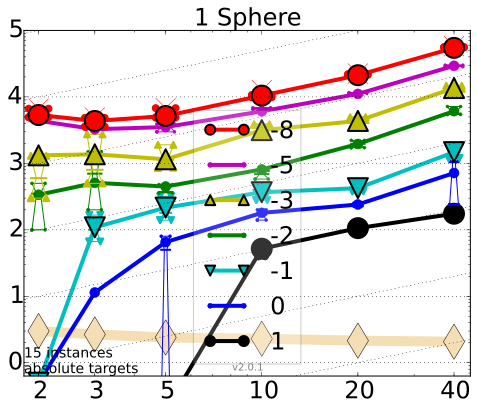
\includegraphics[width=0.266\textwidth]{ppfigdim_f001}&
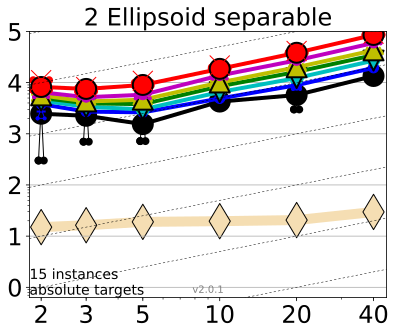
\includegraphics[width=0.266\textwidth]{ppfigdim_f002}&
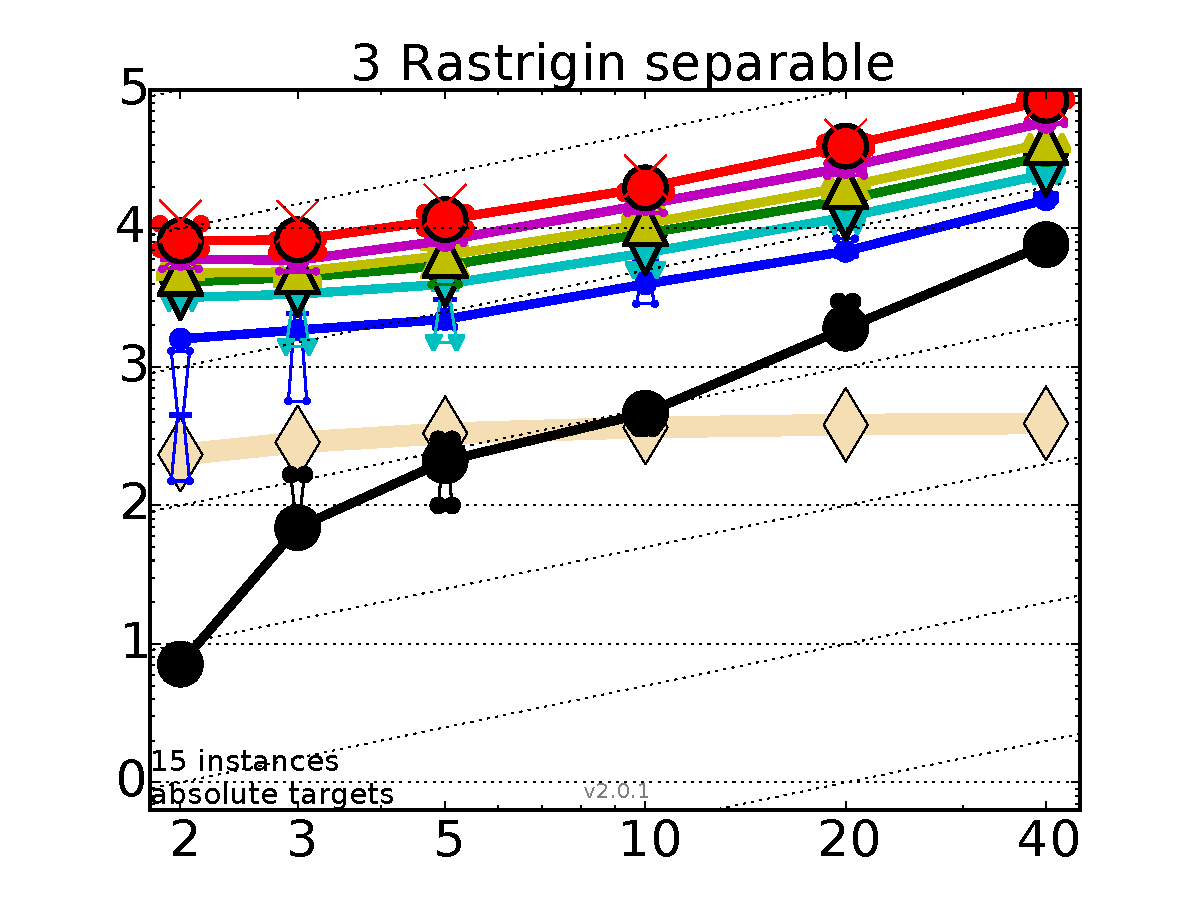
\includegraphics[width=0.266\textwidth]{ppfigdim_f003}&
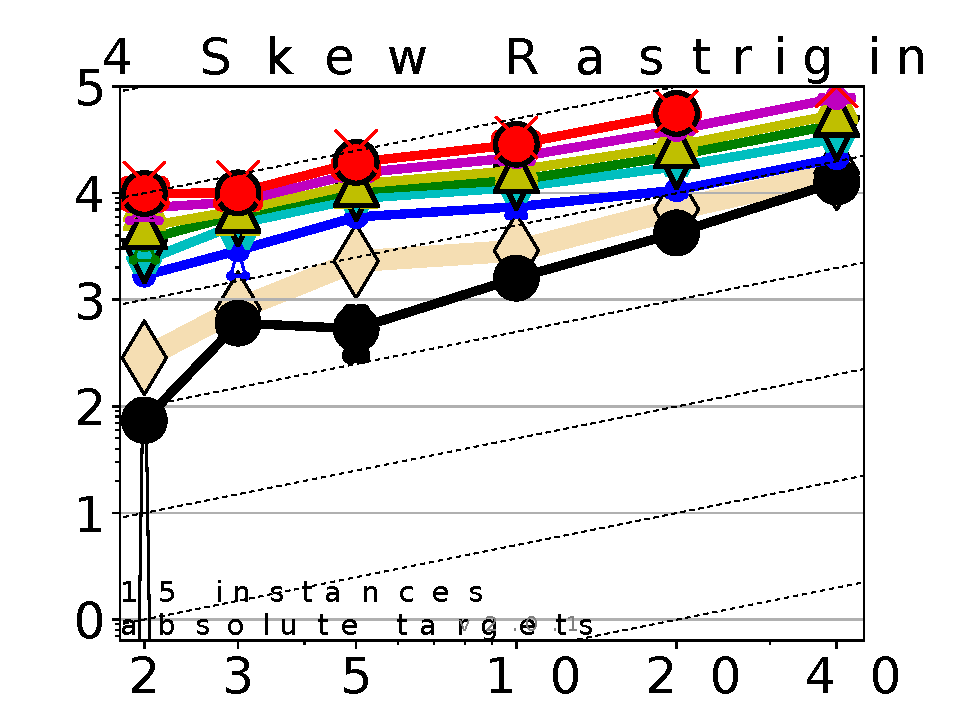
\includegraphics[width=0.266\textwidth]{ppfigdim_f004}\\[-2.1ex]
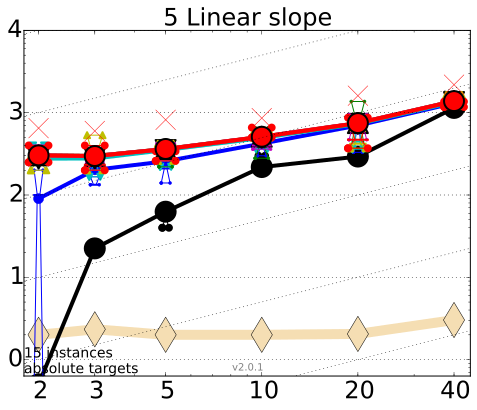
\includegraphics[width=0.266\textwidth]{ppfigdim_f005}&
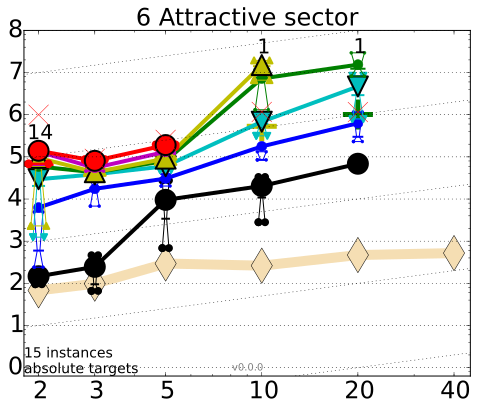
\includegraphics[width=0.266\textwidth]{ppfigdim_f006}&
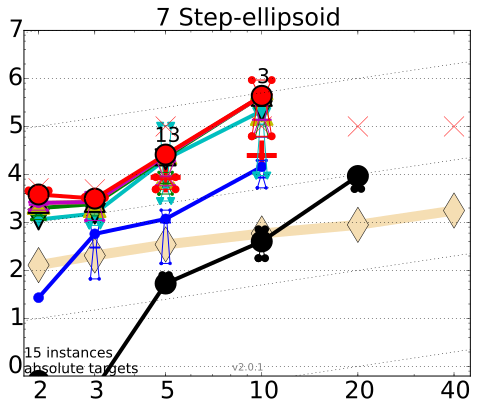
\includegraphics[width=0.266\textwidth]{ppfigdim_f007}&
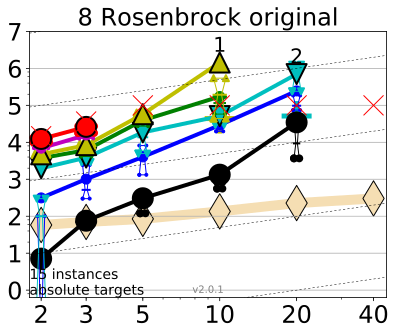
\includegraphics[width=0.266\textwidth]{ppfigdim_f008}\\[-2.1ex]
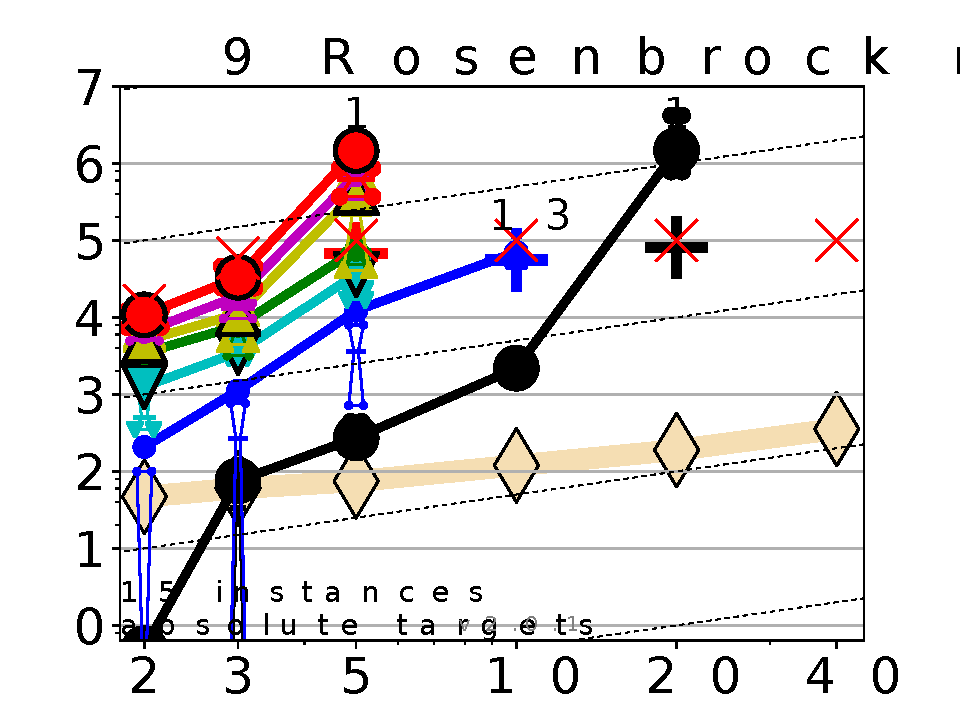
\includegraphics[width=0.266\textwidth]{ppfigdim_f009}&
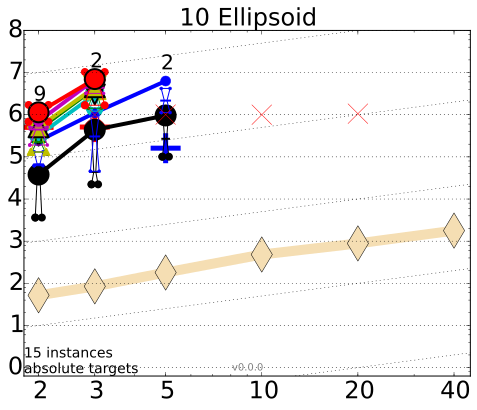
\includegraphics[width=0.266\textwidth]{ppfigdim_f010}&
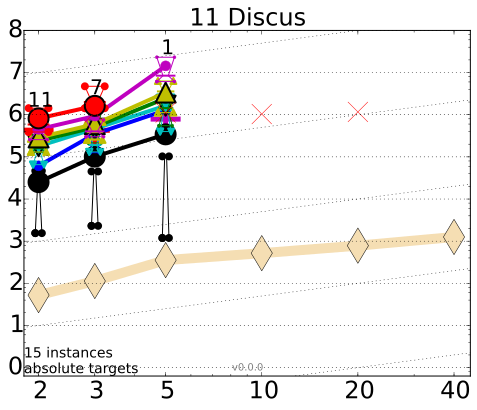
\includegraphics[width=0.266\textwidth]{ppfigdim_f011}&
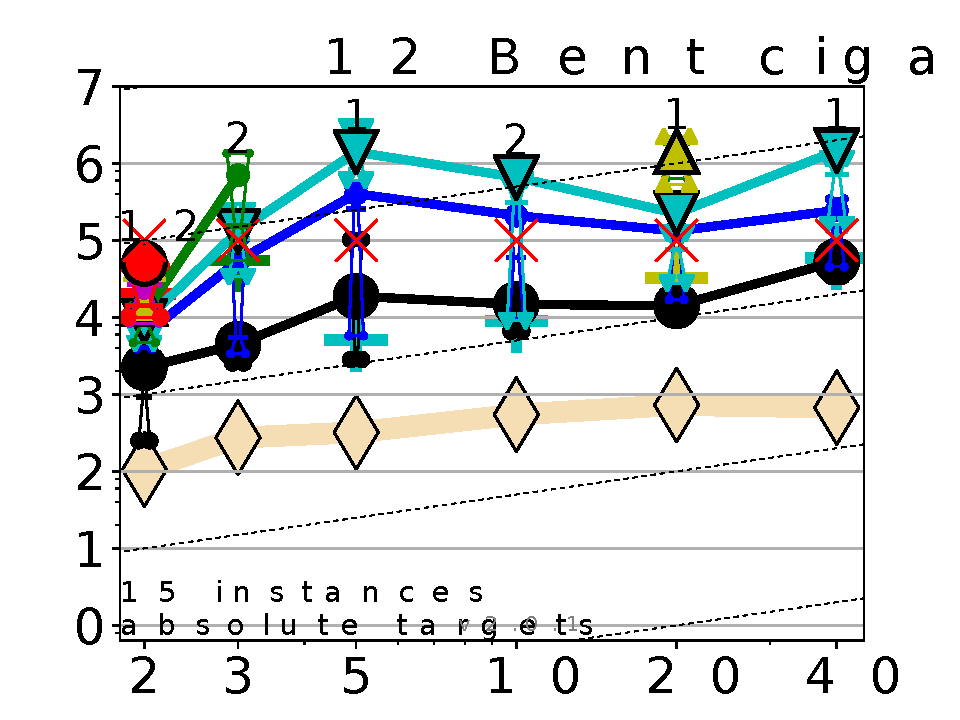
\includegraphics[width=0.266\textwidth]{ppfigdim_f012}\\[-2.1ex]
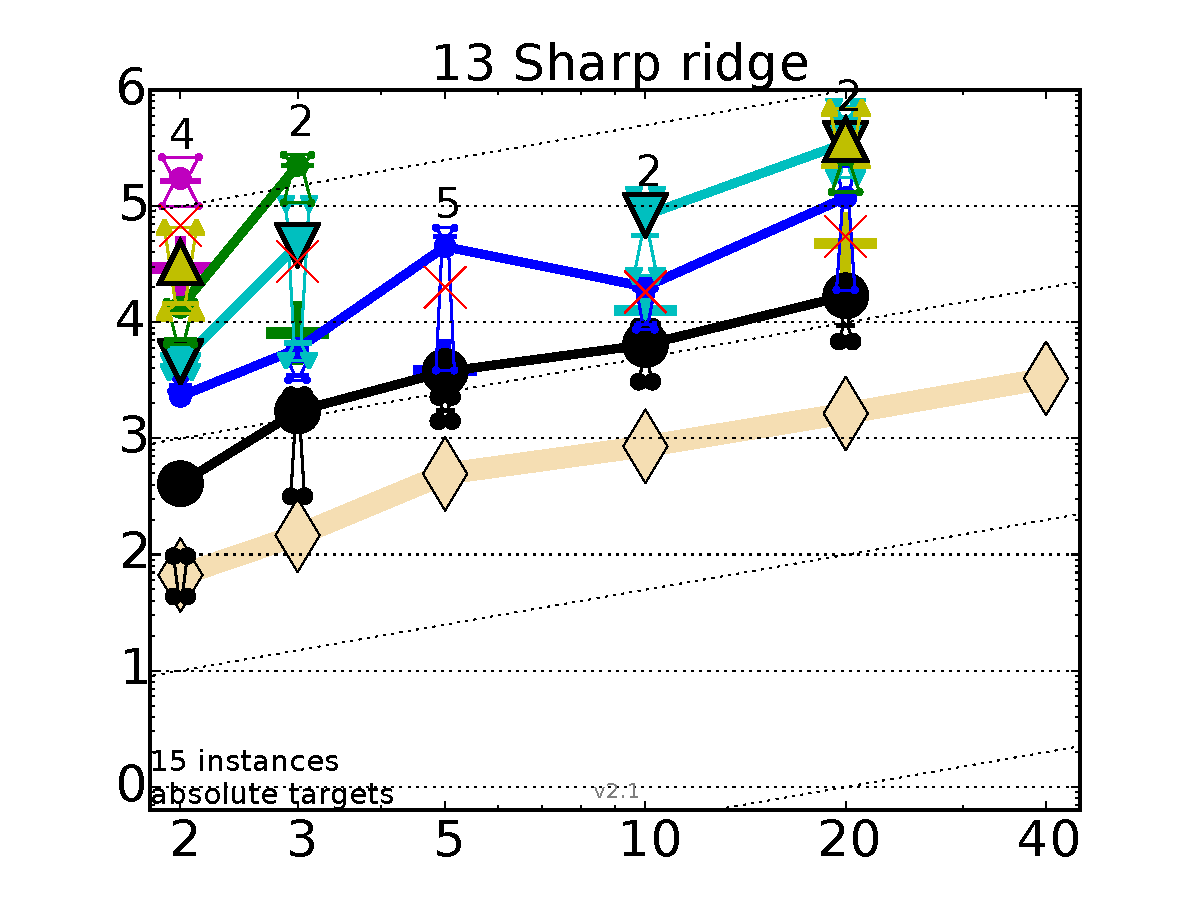
\includegraphics[width=0.266\textwidth]{ppfigdim_f013}&
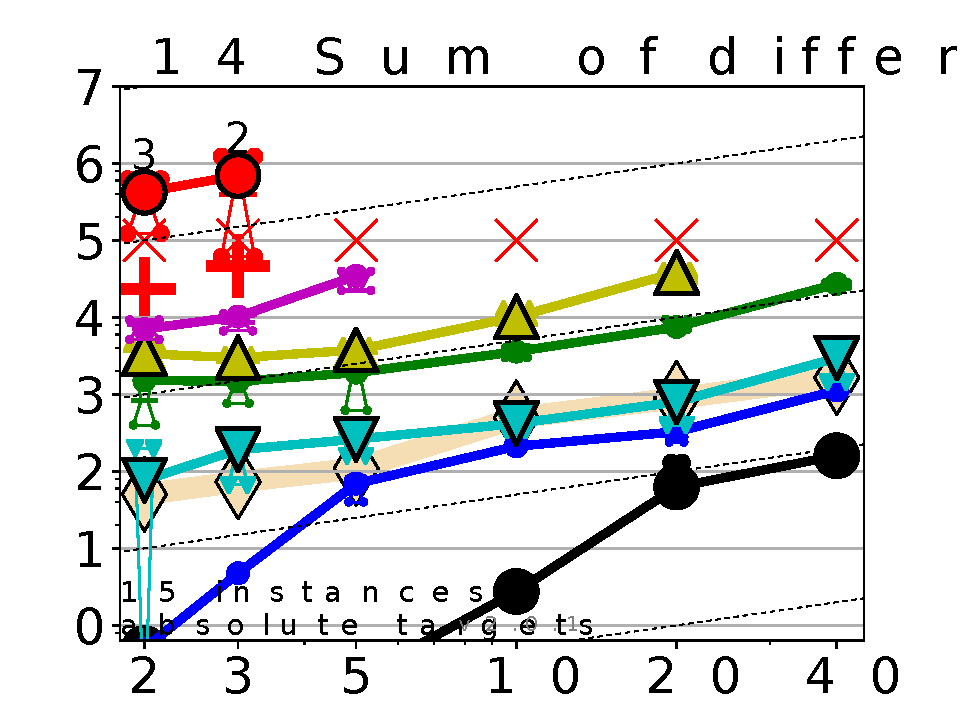
\includegraphics[width=0.266\textwidth]{ppfigdim_f014}&
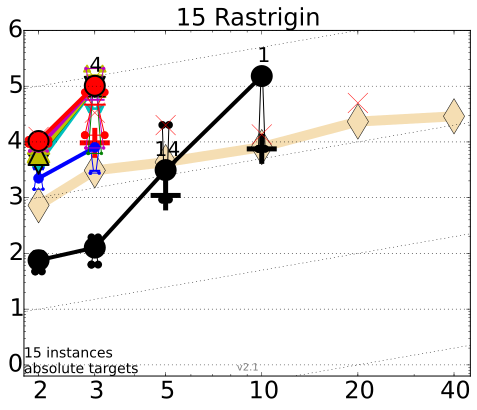
\includegraphics[width=0.266\textwidth]{ppfigdim_f015}&
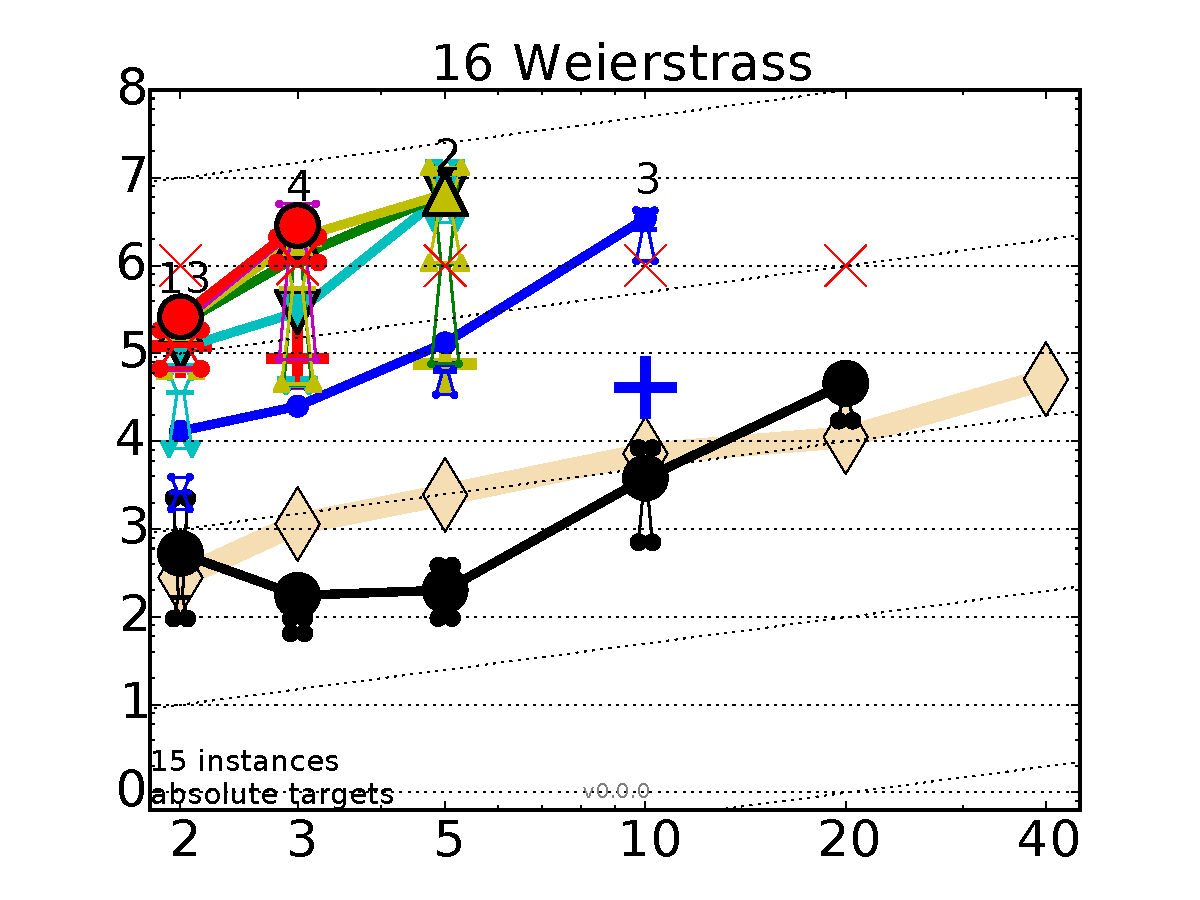
\includegraphics[width=0.266\textwidth]{ppfigdim_f016}\\[-2.1ex]
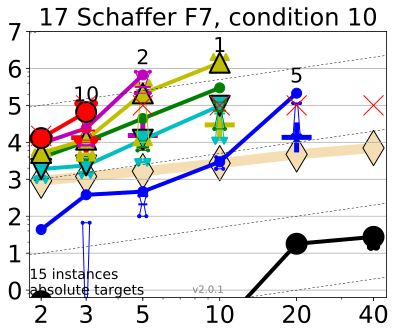
\includegraphics[width=0.266\textwidth]{ppfigdim_f017}&
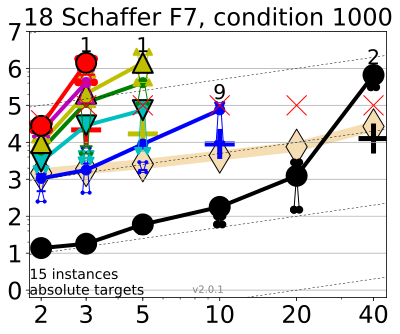
\includegraphics[width=0.266\textwidth]{ppfigdim_f018}&
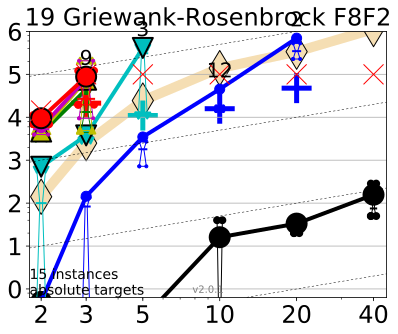
\includegraphics[width=0.266\textwidth]{ppfigdim_f019}&
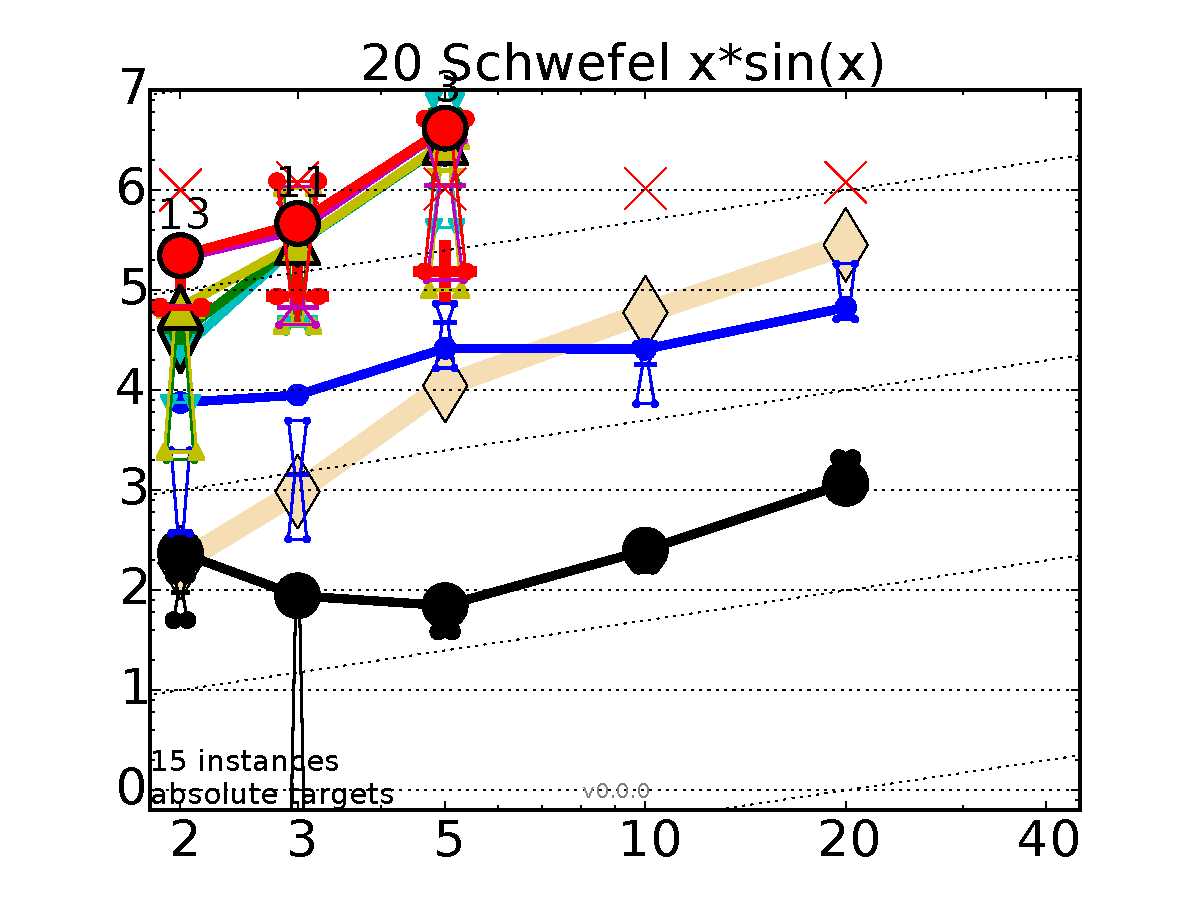
\includegraphics[width=0.266\textwidth]{ppfigdim_f020}\\[-2.1ex]
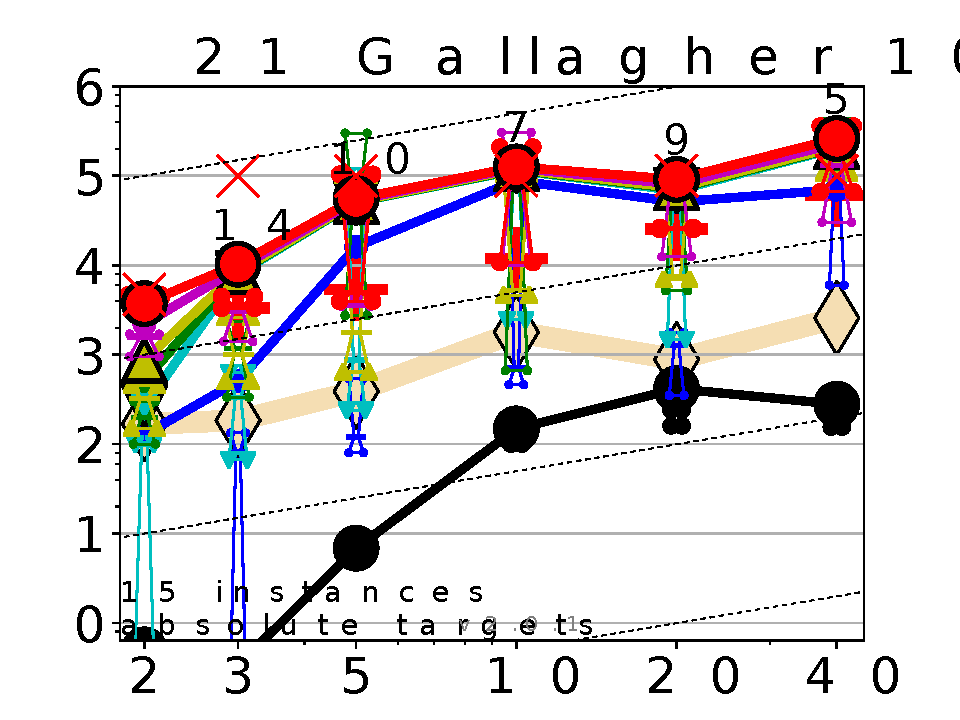
\includegraphics[width=0.266\textwidth]{ppfigdim_f021}&
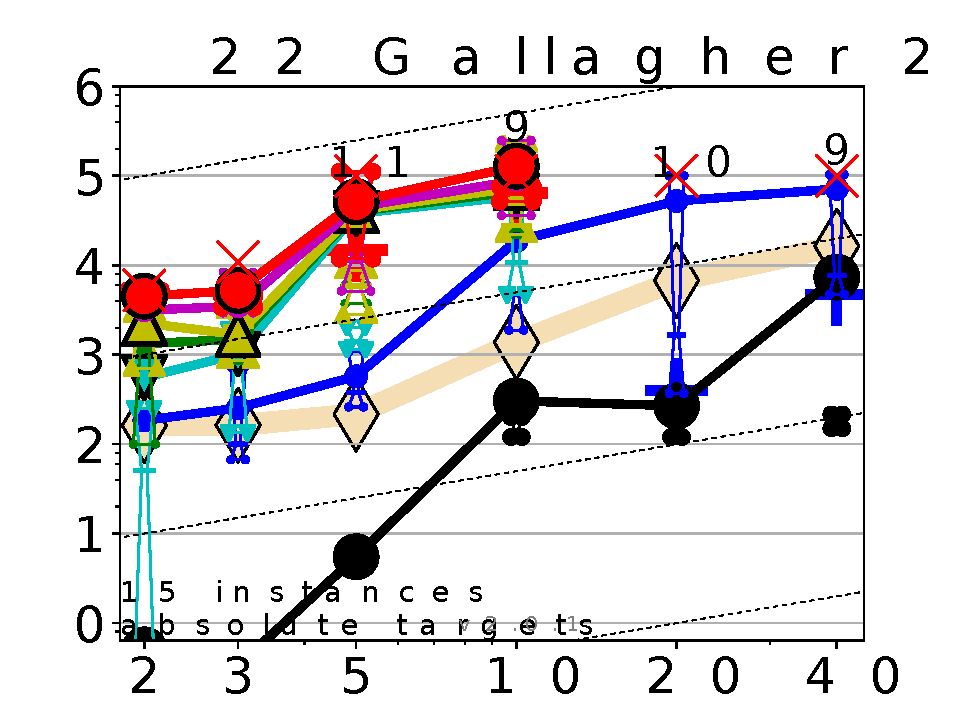
\includegraphics[width=0.266\textwidth]{ppfigdim_f022}&
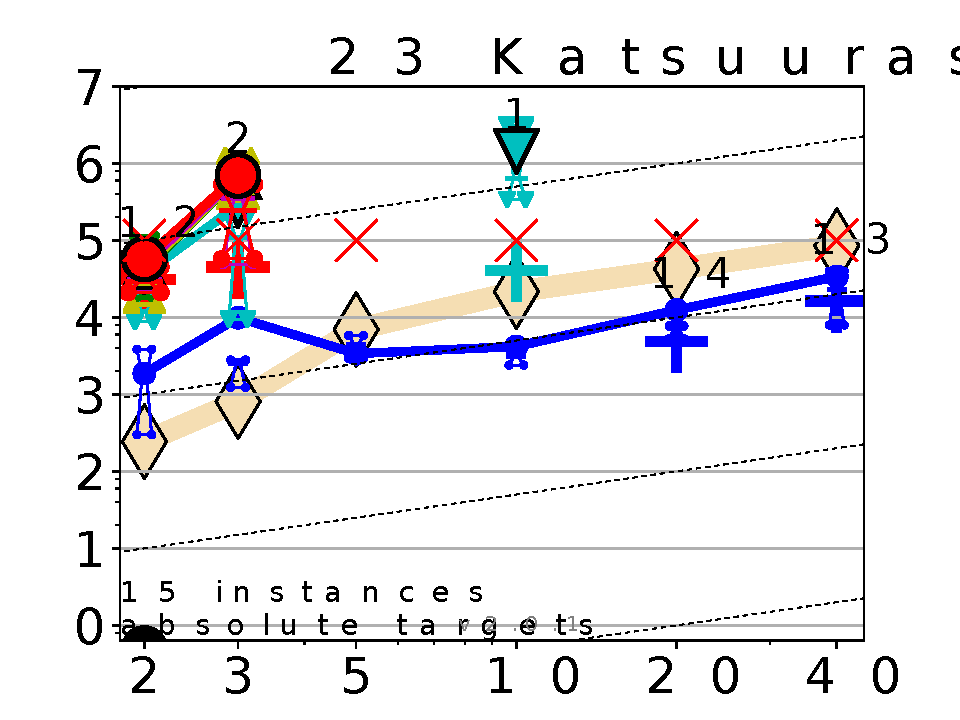
\includegraphics[width=0.266\textwidth]{ppfigdim_f023}&
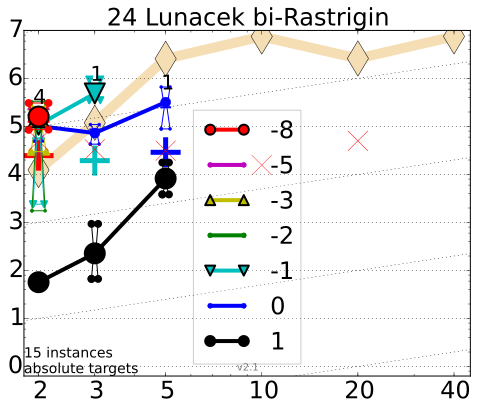
\includegraphics[width=0.266\textwidth]{ppfigdim_f024}
\end{tabular}
\vspace{-3ex}
 \caption{\label{fig:aRTgraphs}
 \bbobppfigdimlegend{$f_1$ and $f_{24}$}
 }
\end{figure*}

%%%%%%%%%%%%%%%%%%%%%%%%%%%%%%%%%%%%%%%%%%%%%%%%%%%%%%%%%%%%%%%%%%%%%%%%%%%%%%%
%%%%%%%%%%%%%%%%%%%%%%%%%%%%%%%%%%%%%%%%%%%%%%%%%%%%%%%%%%%%%%%%%%%%%%%%%%%%%%%
 
% Table showing the average runtime (aRT in number of function
% evaluations) divided by the best aRT measured during BBOB-2009 (given in the
% first row of each cell) for functions $f_1$--$f_{24} for dimension 5$.

%%%%%%%%%%%%%%%%%%%%%%%%%%%%%%%%%%%%%%%%%%%%%%%%%%%%%%%%%%%%%%%%%%%%%%%%%%%%%%%

\begin{table*}\tiny
%\hfill5-D\hfill~\\[1ex]
{\normalsize \color{red}
\ifthenelse{\isundefined{\algorithmG}}{}{more than 6 algorithms: please split the tables below by hand until it fits to the page limits}
}
\mbox{\begin{minipage}[t]{0.499\textwidth}\tiny
\centering
\input{\bbobdatapath\algfolder pptable_header_05D} 

\input{\bbobdatapath\algfolder pptable_f001_05D} 

\input{\bbobdatapath\algfolder pptable_f002_05D}

\input{\bbobdatapath\algfolder pptable_f003_05D}

\input{\bbobdatapath\algfolder pptable_f004_05D}

\input{\bbobdatapath\algfolder pptable_f005_05D}

\input{\bbobdatapath\algfolder pptable_f006_05D}

\input{\bbobdatapath\algfolder pptable_f007_05D}

\input{\bbobdatapath\algfolder pptable_f008_05D}

\input{\bbobdatapath\algfolder pptable_f009_05D}

\input{\bbobdatapath\algfolder pptable_f010_05D}

\input{\bbobdatapath\algfolder pptable_f011_05D}

\input{\bbobdatapath\algfolder pptable_f012_05D}

\end{minipage}
\hspace{0.002\textwidth}
\begin{minipage}[t]{0.499\textwidth}\tiny
\centering
\input{\bbobdatapath\algfolder pptable_header_05D} 

\input{\bbobdatapath\algfolder pptable_f013_05D}

\input{\bbobdatapath\algfolder pptable_f014_05D}

\input{\bbobdatapath\algfolder pptable_f015_05D}

\input{\bbobdatapath\algfolder pptable_f016_05D}

\input{\bbobdatapath\algfolder pptable_f017_05D}

\input{\bbobdatapath\algfolder pptable_f018_05D}

\input{\bbobdatapath\algfolder pptable_f019_05D}

\input{\bbobdatapath\algfolder pptable_f020_05D}

\input{\bbobdatapath\algfolder pptable_f021_05D}

\input{\bbobdatapath\algfolder pptable_f022_05D}

\input{\bbobdatapath\algfolder pptable_f023_05D}

\input{\bbobdatapath\algfolder pptable_f024_05D}
\end{minipage}}

\caption[Table of aRTs]{\label{tab:aRTs5}\bbobpptablecaption{dimension $5$}
}
\end{table*}


%%%%%%%%%%%%%%%%%%%%%%%%%%%%%%%%%%%%%%%%%%%%%%%%%%%%%%%%%%%%%%%%%%%%%%%%%%%%%%%
%%%%%%%%%%%%%%%%%%%%%%%%%%%%%%%%%%%%%%%%%%%%%%%%%%%%%%%%%%%%%%%%%%%%%%%%%%%%%%%

% Table showing the average runtime (aRT in number of function
% evaluations) divided by the best aRT measured during BBOB-2009 (given in the
% first row of each cell) for functions $f_1$--$f_{24} for dimension 20$.

%%%%%%%%%%%%%%%%%%%%%%%%%%%%%%%%%%%%%%%%%%%%%%%%%%%%%%%%%%%%%%%%%%%%%%%%%%%%%%%
\begin{table*}\tiny
%\hfill20-D\hfill~\\[1ex]
\mbox{\begin{minipage}[t]{0.499\textwidth}\tiny
\centering
\input{\bbobdatapath\algfolder pptable_header_20D} 

\input{\bbobdatapath\algfolder pptable_f001_20D} 

\input{\bbobdatapath\algfolder pptable_f002_20D}

\input{\bbobdatapath\algfolder pptable_f003_20D}

\input{\bbobdatapath\algfolder pptable_f004_20D}

\input{\bbobdatapath\algfolder pptable_f005_20D}

\input{\bbobdatapath\algfolder pptable_f006_20D}

\input{\bbobdatapath\algfolder pptable_f007_20D}

\input{\bbobdatapath\algfolder pptable_f008_20D}

\input{\bbobdatapath\algfolder pptable_f009_20D}

\input{\bbobdatapath\algfolder pptable_f010_20D}

\input{\bbobdatapath\algfolder pptable_f011_20D}

\input{\bbobdatapath\algfolder pptable_f012_20D}
\end{minipage}
\hspace{0.002\textwidth}
\begin{minipage}[t]{0.499\textwidth}\tiny
\centering
\input{\bbobdatapath\algfolder pptable_header_20D} 

\input{\bbobdatapath\algfolder pptable_f013_20D}

\input{\bbobdatapath\algfolder pptable_f014_20D}

\input{\bbobdatapath\algfolder pptable_f015_20D}

\input{\bbobdatapath\algfolder pptable_f016_20D}

\input{\bbobdatapath\algfolder pptable_f017_20D}

\input{\bbobdatapath\algfolder pptable_f018_20D}

\input{\bbobdatapath\algfolder pptable_f019_20D}

\input{\bbobdatapath\algfolder pptable_f020_20D}

\input{\bbobdatapath\algfolder pptable_f021_20D}

\input{\bbobdatapath\algfolder pptable_f022_20D}

\input{\bbobdatapath\algfolder pptable_f023_20D}

\input{\bbobdatapath\algfolder pptable_f024_20D}
\end{minipage}}
 
\caption[Table of aRTs]{\label{tab:aRTs20}\bbobpptablecaption{dimension $20$}
}
\end{table*}

%%%%%%%%%%%%%%%%%%%%%%%%%%%%%%%%%%%%%%%%%%%%%%%%%%%%%%%%%%%%%%%%%%%%%%%%%%%%%%%


%%%%%%%%%%%%%%%%%%%%%%%%%%%%%%%%%%%%%%%%%%%%%%%%%%%%%%%%%%%%%%%%%%%%%%%%%%%%%%%
%%%%%%%%%%%%%%%%%%%%%%%%%%%%%%%%%%%%%%%%%%%%%%%%%%%%%%%%%%%%%%%%%%%%%%%%%%%%%%%

% Empirical cumulative distribution functions (ECDFs) per function group.

%%%%%%%%%%%%%%%%%%%%%%%%%%%%%%%%%%%%%%%%%%%%%%%%%%%%%%%%%%%%%%%%%%%%%%%%%%%%%%%
\newcommand{\rot}[2][2.5]{
  \hspace*{-3.5\baselineskip}%
  \begin{rotate}{90}\hspace{#1em}#2
  \end{rotate}}
\begin{figure*}
\begin{tabular}{l@{\hspace*{-0.025\textwidth}}l@{\hspace*{-0.00\textwidth}}|l@{\hspace*{-0.025\textwidth}}l}
\multicolumn{2}{c}{$D=5$} & \multicolumn{2}{c}{$D=20$}\\[-0.5ex]
\rot{separable fcts}
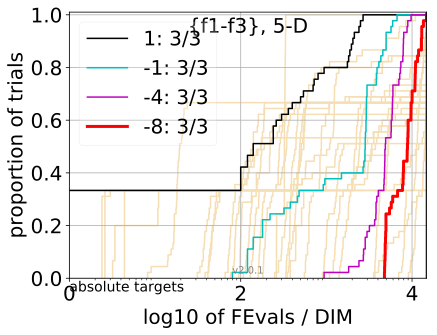
\includegraphics[width=0.268\textwidth,trim=0 0 0 13mm, clip]{pprldistr_05D_separ} &
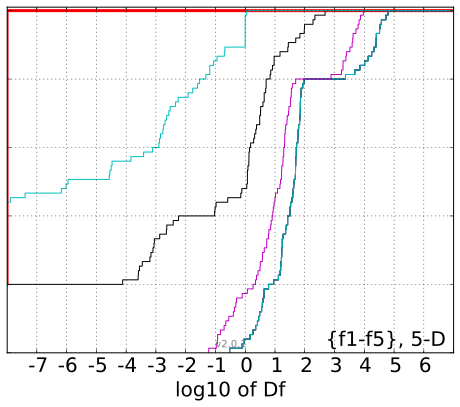
\includegraphics[width=0.2362\textwidth,trim=2.40cm 0 0 13mm, clip]{ppfvdistr_05D_separ} &
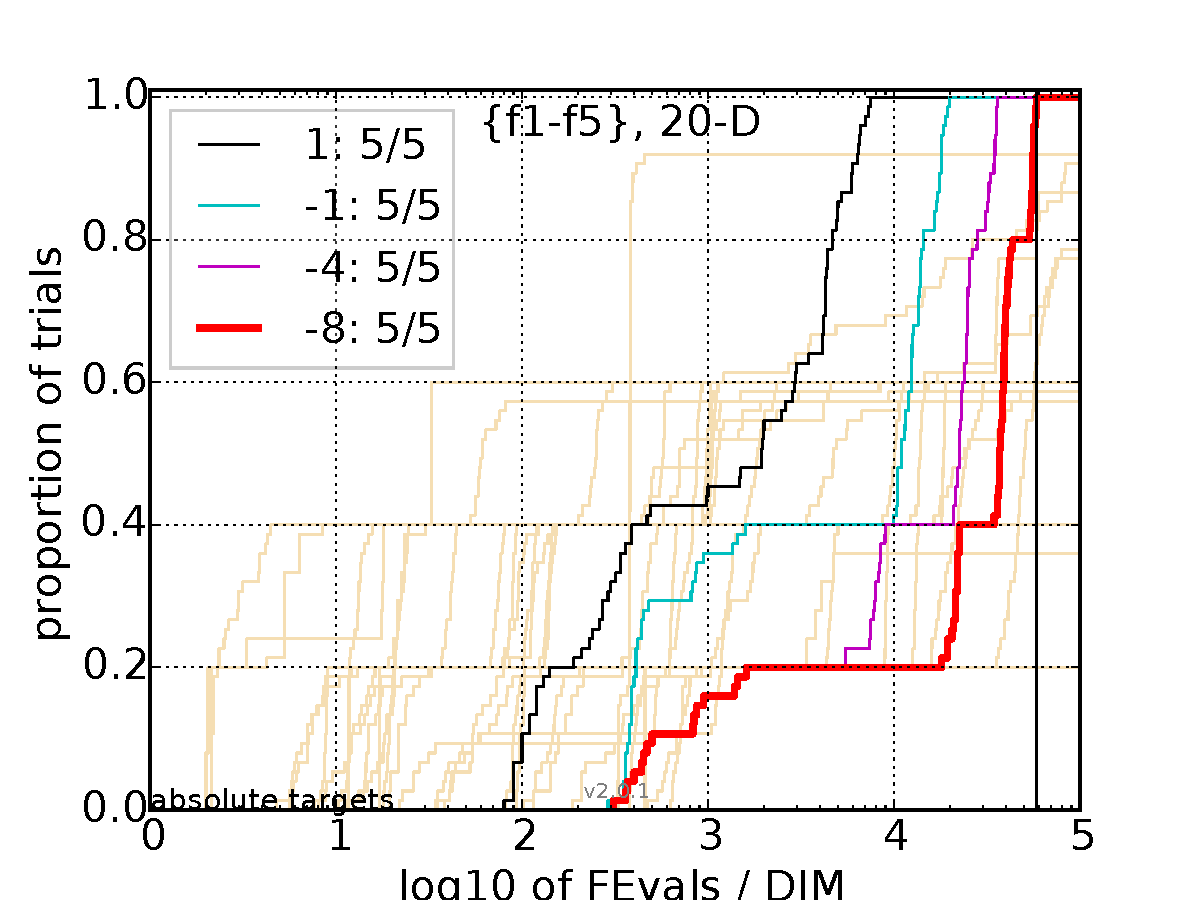
\includegraphics[width=0.268\textwidth,trim=0 0 0 13mm, clip]{pprldistr_20D_separ} &
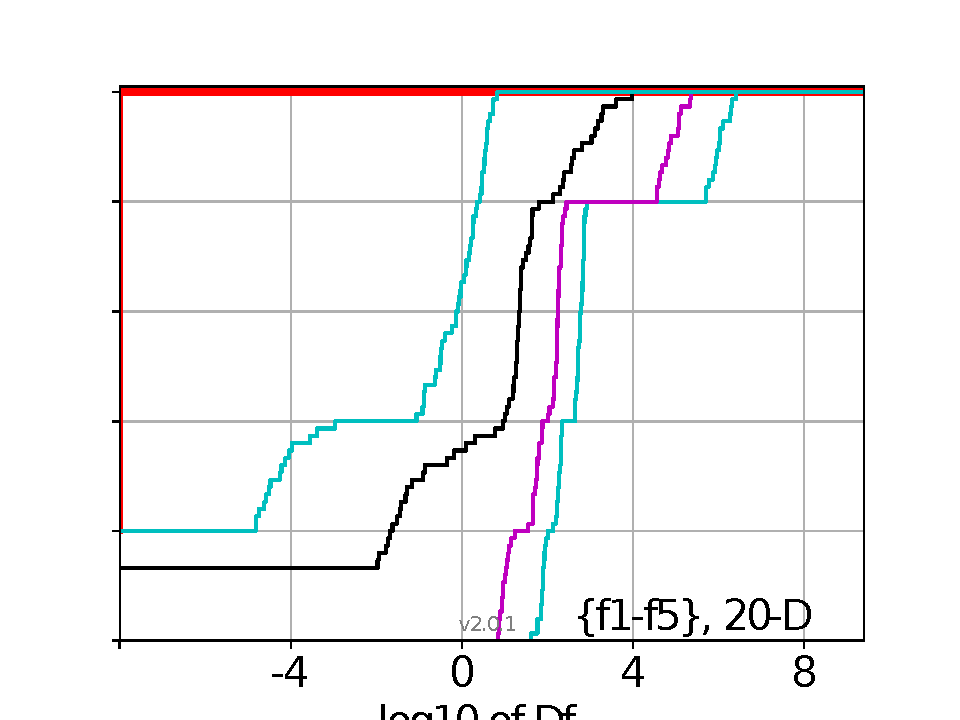
\includegraphics[width=0.2362\textwidth,trim=2.40cm 0 0 13mm, clip]{ppfvdistr_20D_separ} \\[-2ex]
\rot[1]{misc.\ moderate fcts}
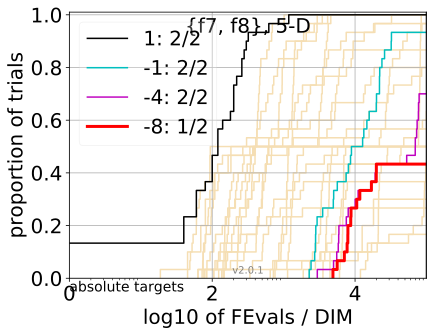
\includegraphics[width=0.268\textwidth,trim=0 0 0 13mm, clip]{pprldistr_05D_lcond} &
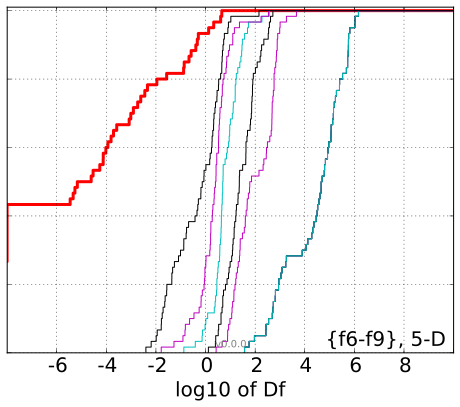
\includegraphics[width=0.2362\textwidth,trim=2.40cm 0 0 13mm, clip]{ppfvdistr_05D_lcond} &
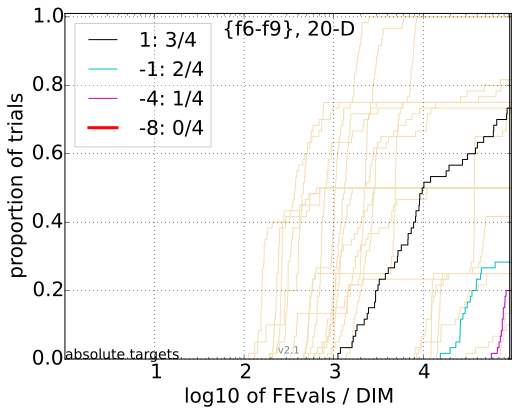
\includegraphics[width=0.268\textwidth,trim=0 0 0 13mm, clip]{pprldistr_20D_lcond} &
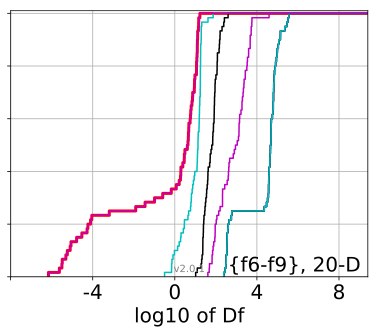
\includegraphics[width=0.2362\textwidth,trim=2.40cm 0 0 13mm, clip]{ppfvdistr_20D_lcond} \\[-2ex]
\rot[1.3]{ill-conditioned fcts}
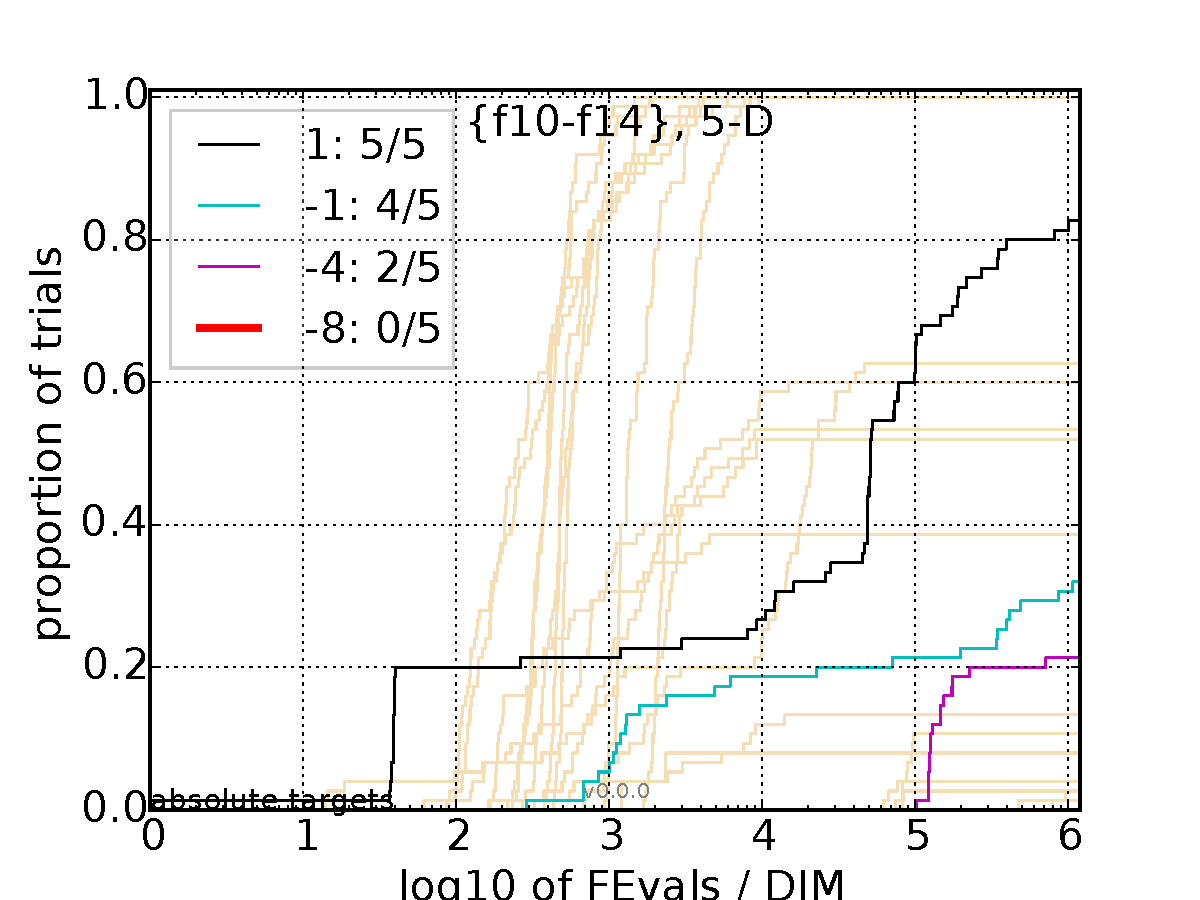
\includegraphics[width=0.268\textwidth,trim=0 0 0 13mm, clip]{pprldistr_05D_hcond} &
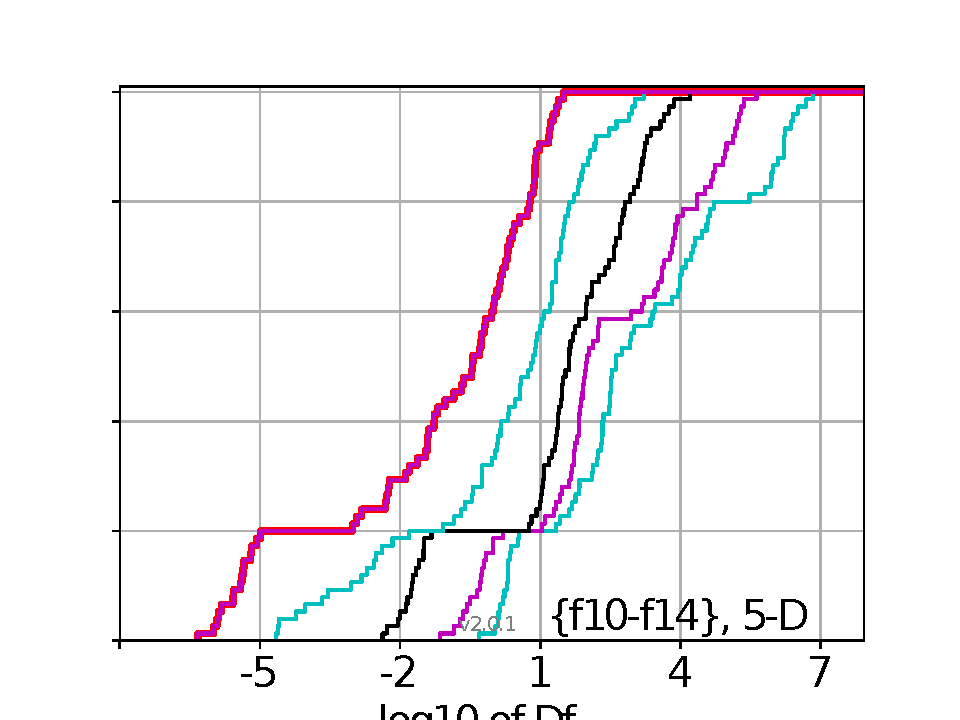
\includegraphics[width=0.2362\textwidth,trim=2.40cm 0 0 13mm, clip]{ppfvdistr_05D_hcond} &
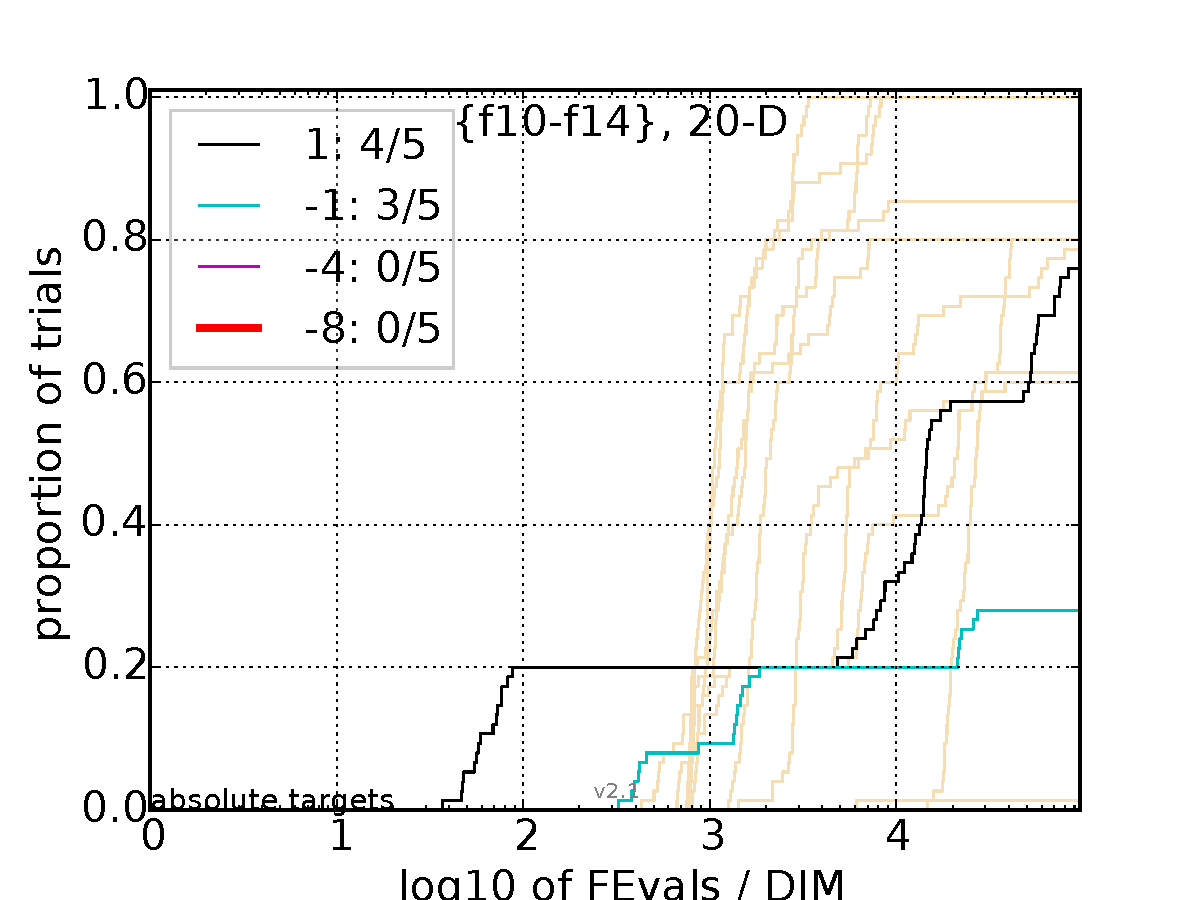
\includegraphics[width=0.268\textwidth,trim=0 0 0 13mm, clip]{pprldistr_20D_hcond} &
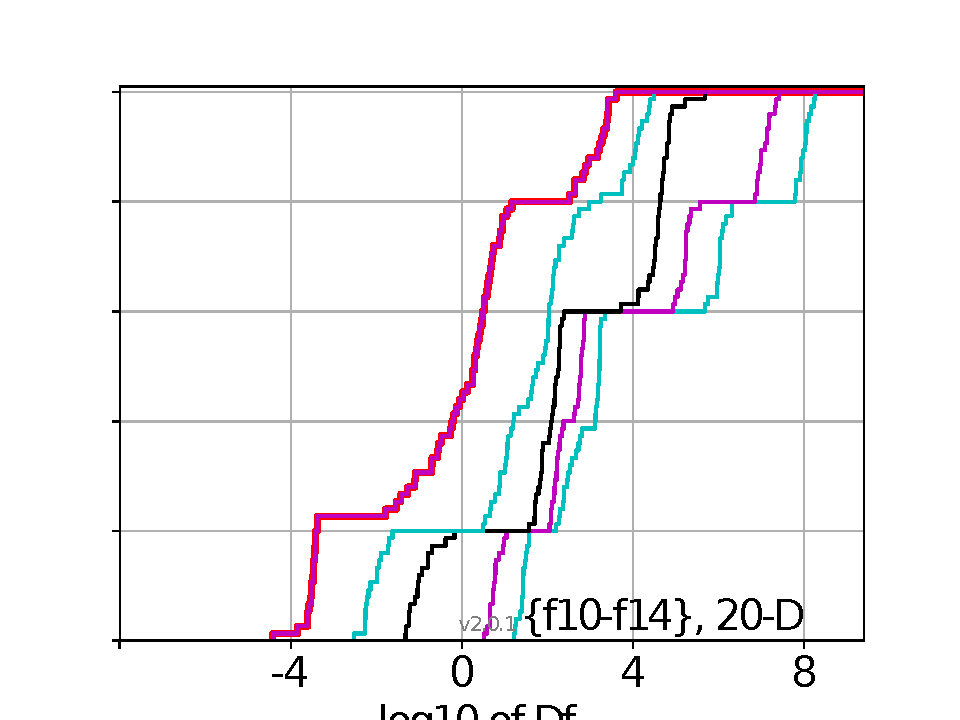
\includegraphics[width=0.2362\textwidth,trim=2.40cm 0 0 13mm, clip]{ppfvdistr_20D_hcond} \\[-2ex]
\rot[1.6]{multi-modal fcts}
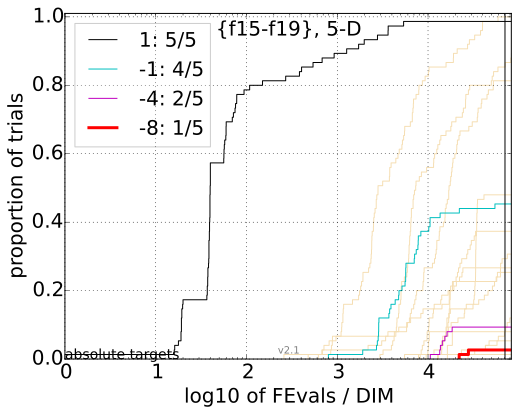
\includegraphics[width=0.268\textwidth,trim=0 0 0 13mm, clip]{pprldistr_05D_multi} &
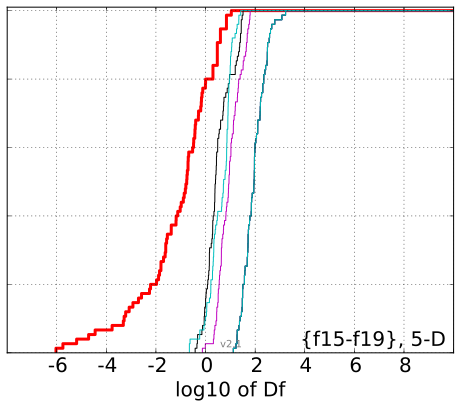
\includegraphics[width=0.2362\textwidth,trim=2.40cm 0 0 13mm, clip]{ppfvdistr_05D_multi} &
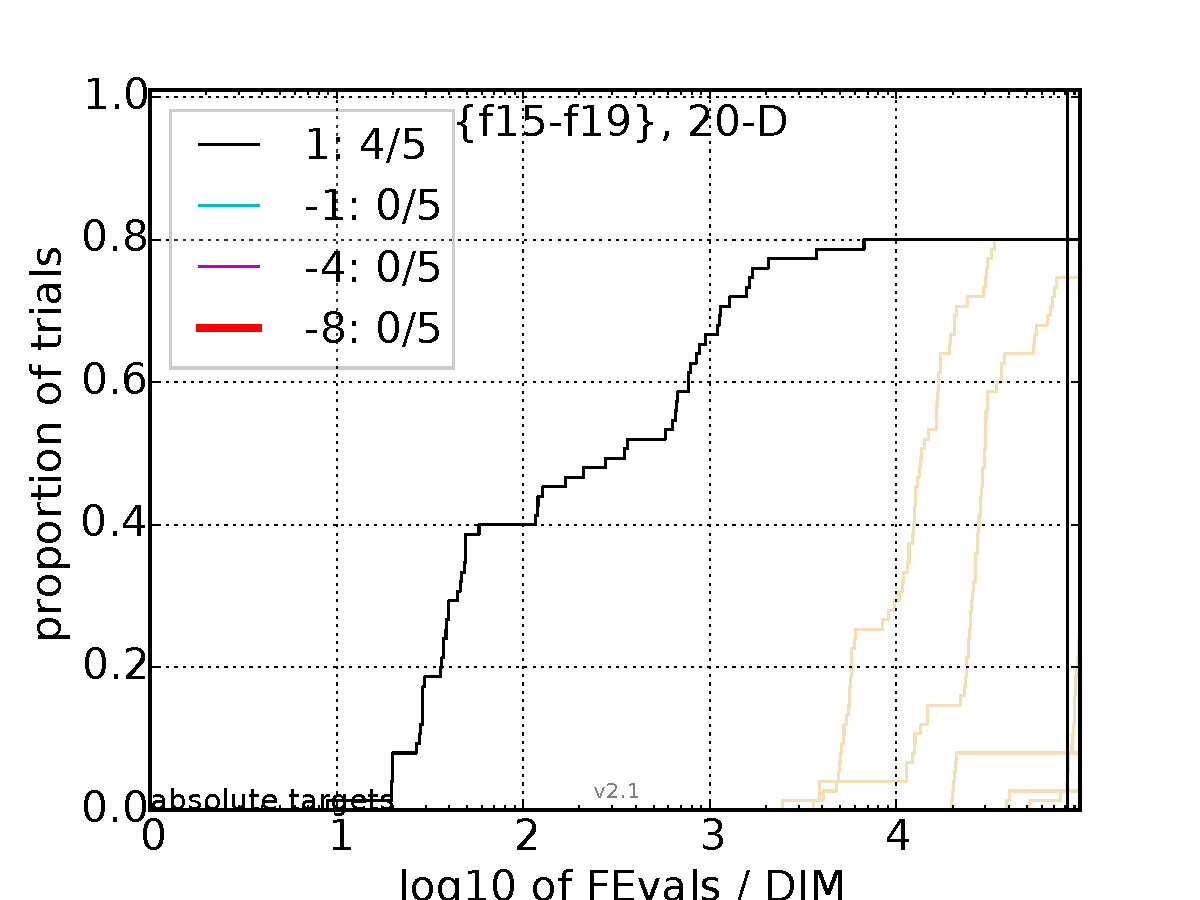
\includegraphics[width=0.268\textwidth,trim=0 0 0 13mm, clip]{pprldistr_20D_multi} &
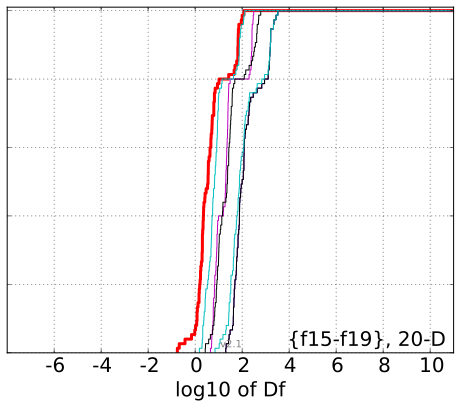
\includegraphics[width=0.2362\textwidth,trim=2.40cm 0 0 13mm, clip]{ppfvdistr_20D_multi} \\[-2ex]
\rot[1.0]{weak structure fcts}
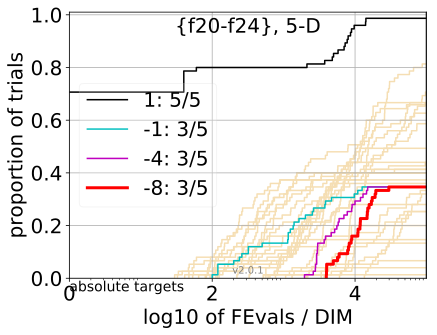
\includegraphics[width=0.268\textwidth,trim=0 0 0 13mm, clip]{pprldistr_05D_mult2} &
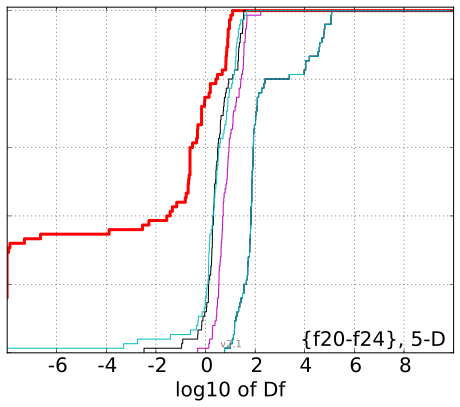
\includegraphics[width=0.2362\textwidth,trim=2.40cm 0 0 13mm, clip]{ppfvdistr_05D_mult2} &
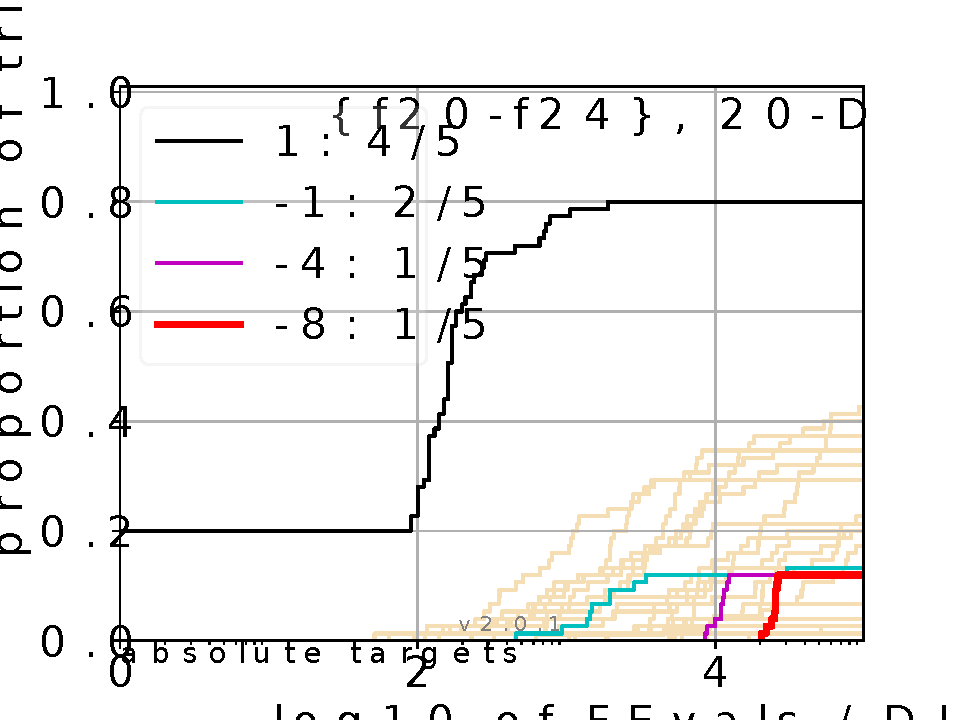
\includegraphics[width=0.268\textwidth,trim=0 0 0 13mm, clip]{pprldistr_20D_mult2} &
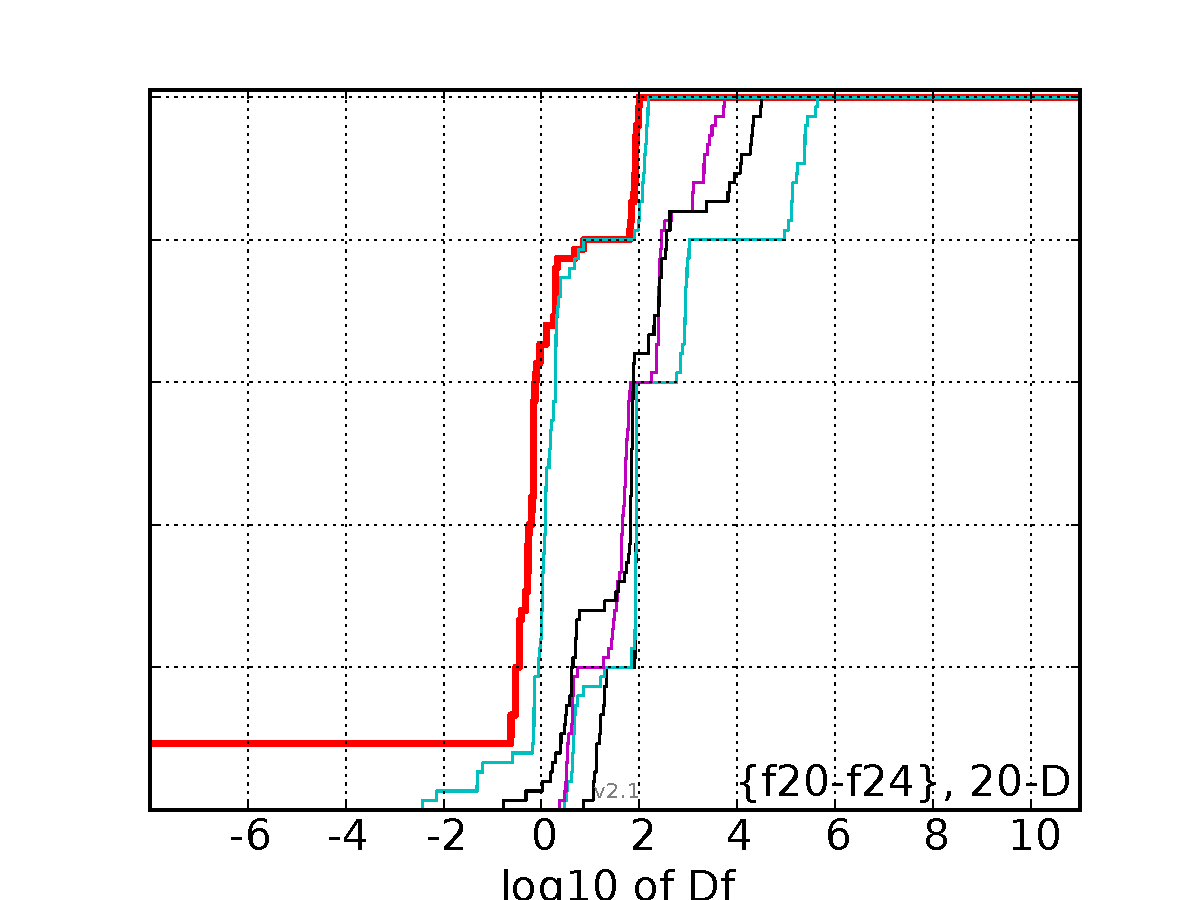
\includegraphics[width=0.2362\textwidth,trim=2.40cm 0 0 13mm, clip]{ppfvdistr_20D_mult2}\\[-2ex]
\rot{all functions}
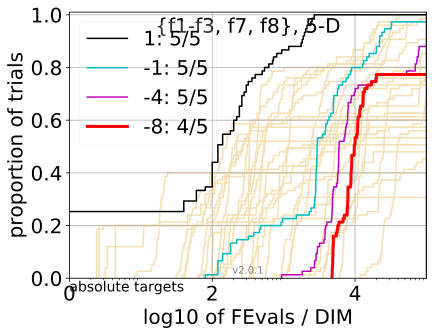
\includegraphics[width=0.268\textwidth,trim=0 0 0 13mm, clip]{pprldistr_05D_noiselessall} &
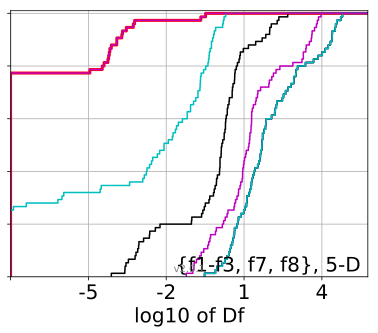
\includegraphics[width=0.2362\textwidth,trim=2.40cm 0 0 13mm, clip]{ppfvdistr_05D_noiselessall} &
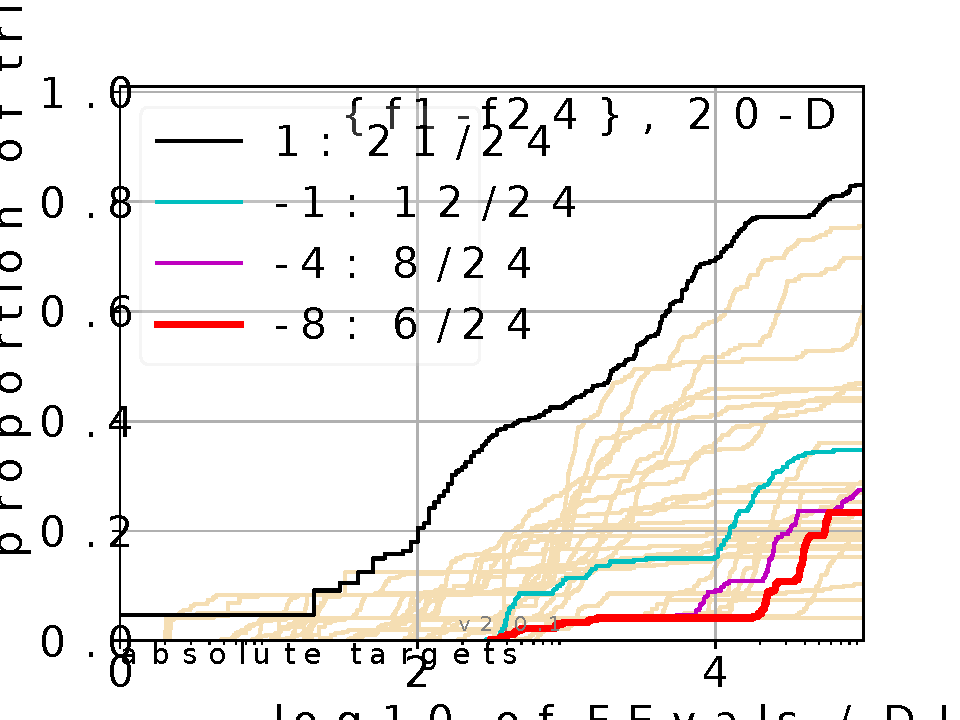
\includegraphics[width=0.268\textwidth,trim=0 0 0 13mm, clip]{pprldistr_20D_noiselessall} &
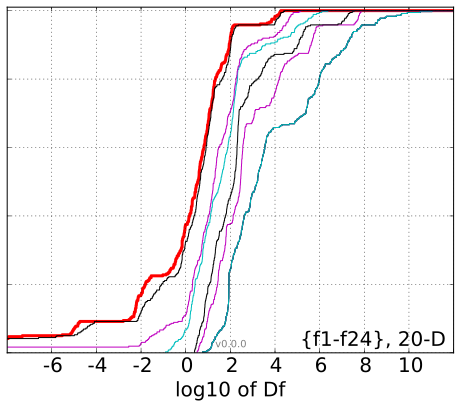
\includegraphics[width=0.2362\textwidth,trim=2.40cm 0 0 13mm, clip]{ppfvdistr_20D_noiselessall}
\vspace*{-0.5ex}
\end{tabular}
 \caption{\label{fig:RLDs}
 \bbobpprldistrlegend{}
 }
\end{figure*}
%%%%%%%%%%%%%%%%%%%%%%%%%%%%%%%%%%%%%%%%%%%%%%%%%%%%%%%%%%%%%%%%%%%%%%%%%%%%%%%


%%%%%%%%%%%%%%%%%%%%%%%%%%%%%%%%%%%%%%%%%%%%%%%%%%%%%%%%%%%%%%%%%%%%%%%%%%%%%%%
%%%%%%%%%%%%%%%%%%%%%%%%%%%%%%%%%%%%%%%%%%%%%%%%%%%%%%%%%%%%%%%%%%%%%%%%%%%%%%%

% aRT loss ratios (figure and table)

%%%%%%%%%%%%%%%%%%%%%%%%%%%%%%%%%%%%%%%%%%%%%%%%%%%%%%%%%%%%%%%%%%%%%%%%%%%%%%%
\begin{figure}
\centering
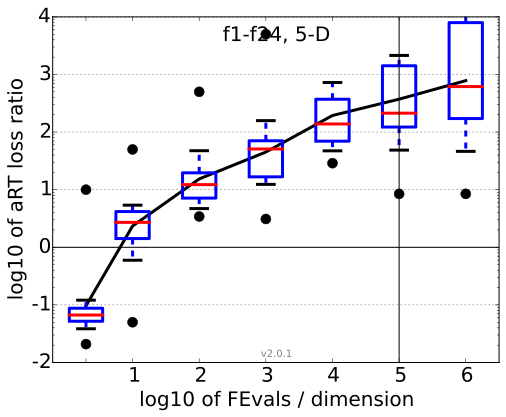
\includegraphics[width=0.24\textwidth,trim=0 0 16mm 12mm, clip]{pplogloss_05D_noiselessall}% 
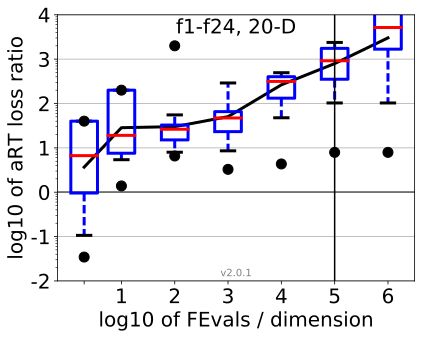
\includegraphics[width=0.24\textwidth,trim=7mm 0 9mm 12mm, clip]{pplogloss_20D_noiselessall}%
\\[-6.2ex]
\parbox{0.49\columnwidth}{\centering 5-D}%
\parbox{0.49\columnwidth}{\centering 20-D}\\[5ex]
%
\input{\bbobdatapath\algfolder pploglosstable_05D_noiselessall}\\
\input{\bbobdatapath\algfolder pploglosstable_20D_noiselessall}
\caption{\label{tab:aRTloss}%
\bbobloglosstablecaption{}
}
\end{figure}


%%%%%%%%%%%%%%%%%%%%%%%%%%%%%%%%%%%%%%%%%%%%%%%%%%%%%%%%%%%%%%%%%%%%%%%%%%%%%%%
%%%%%%%%%%%%%%%%%%%%%%%%%%%%%%%%%%%%%%%%%%%%%%%%%%%%%%%%%%%%%%%%%%%%%%%%%%%%%%%

% aRT loss ratios per function group

%%%%%%%%%%%%%%%%%%%%%%%%%%%%%%%%%%%%%%%%%%%%%%%%%%%%%%%%%%%%%%%%%%%%%%%%%%%%%%%
\begin{figure}
\begin{tabular}{@{}l@{}@{}l@{}}
\multicolumn{1}{c}{5-D} & \multicolumn{1}{c}{20-D}\\
%\rot{all functions}
%\hspace*{-2mm}
\rot{separable fcts}
\hspace*{-1.4mm}
\includegraphics[width=0.24\textwidth,trim=0 0 16mm 12mm, clip]{pplogloss_05D_separ} &
\includegraphics[width=0.24\textwidth,trim=7mm 0 9mm 12mm, clip]{pplogloss_20D_separ}\\[-2ex]
\rot[2]{moderate fcts}
\hspace*{-1.4mm}
\includegraphics[width=0.24\textwidth,trim=0 0 16mm 12mm, clip]{pplogloss_05D_lcond} &
\includegraphics[width=0.24\textwidth,trim=7mm 0 9mm 12mm, clip]{pplogloss_20D_lcond}\\[-2ex]
\rot[1.3]{ill-conditioned fcts}
\hspace*{-1.4mm}
\includegraphics[width=0.24\textwidth,trim=0 0 16mm 12mm, clip]{pplogloss_05D_hcond} &
\includegraphics[width=0.24\textwidth,trim=7mm 0 9mm 12mm, clip]{pplogloss_20D_hcond}\\[-2ex]
\rot[1.6]{multi-modal fcts}
\hspace*{-1.4mm}
\includegraphics[width=0.24\textwidth,trim=0 0 16mm 12mm, clip]{pplogloss_05D_multi} &
\includegraphics[width=0.24\textwidth,trim=7mm 0 9mm 12mm, clip]{pplogloss_20D_multi}\\[-2ex]
\rot[1.0]{weak structure fcts}
\hspace*{-1.4mm}
\includegraphics[width=0.24\textwidth,trim=0 0 16mm 12mm, clip]{pplogloss_05D_mult2} &
\includegraphics[width=0.24\textwidth,trim=7mm 0 9mm 12mm, clip]{pplogloss_20D_mult2}
\vspace*{-0.5ex}
\end{tabular}
 \caption{\label{fig:aRTlogloss}%
\bbobloglossfigurecaption{}
}
\end{figure}

%%%%%%%%%%%%%%%%%%%%%%%%%%%%%%%%%%%%%%%%%%%%%%%%%%%%%%%%%%%%%%%%%%%%%%%%%%%%%%%


%%%%%%%%%%%%%%%%%%%%%%%%%%%%%%%%%%%%%%%%%%%%%%%%%%%%%%%%%%%%%%%%%%%%%%%%%%%%%%%
\section{Discussion}  % and or conclusion, summary...
%%%%%%%%%%%%%%%%%%%%%%%%%%%%%%%%%%%%%%%%%%%%%%%%%%%%%%%%%%%%%%%%%%%%%%%%%%%%%%%
The results obtained show that an asynchronous execution 
following a Pool-based approach is  possible and easy to achieve.
Results, however, are still preliminary and further tuning of the parameters could 
potentially wield better results.

Future lines of work will focus on using other EA or 
meta-heuristic techniques, such as the Grey Wolf Optimizer \cite{mirjalili2014grey}
or Differential Evolution \cite{storn1997differential} for having workers that are 
heterogeneous in more than one sense. RPSS could be used 
in those cases where each algorithm has a different set of 
parameters, but also to randomly select the technique employed. 

\bibliographystyle{ACM-Reference-Format}
%\bibliography{bbob}  % bbob.bib is the name of the Bibliography in this case
\bibliography{../bib/biblio,../bib/evospace-i,../bib/parameters,../bib/volunteer,../bib/geneura,../bib/pool,bbob} 

\clearpage % otherwise the last figure might be missing

\end{document}